\chapter{函数与函数类的逼近}
\label{chap:function-approximation}

计算机只能存储有限个数。要在计算中使用$[0,1]$上的折线$f_*(x)=|x-1/2|$，可以记下多项式的系数、样条在结点处的值，或者一个小网络的权重；它们都用有限个数描述一个近似函数。由此产生三个问题。第一，固定目标、定义域和误差范数后，哪些有限表示能把误差压到任意小，误差又怎样随次数、结点数或单元数下降？第二，目标有多个变量时，表示所需的数目怎样随维数增长，能否利用变量之间的分离结构减少数目？第三，若事先只知道目标属于某个函数类，例如全体以$1$为Lipschitz常数、绝对值不超过$1$的函数，能否预先备好有限个代表，使类中每个成员都靠近其中之一，又至少需要多少个代表？

前三个问题依次改变了被逼近的对象。第~\ref{sec:apx-single-function}节固定一个目标，比较多项式、样条、核截面和神经单元四种生成方式；它们的预算可以随精度增加，结论分为“能否任意逼近”和“误差下降多快”两类，后者总要额外的光滑性。第~\ref{sec:apx-multivariate}节固定变量的分组方式，研究由单变量函数组成多变量函数的张量积空间，以及只用少数乘积项的低秩表示。第~\ref{sec:apx-function-classes}节把对象从单个函数换成整个函数类，量词随之改变：每个成员各有一个近似，不等于一套共同的有限代表适用于全体。为此先用Arzelà--Ascoli判据刻画一致距离下的相对紧性，再用覆盖数计量所需代表的个数。

本章使用第~\ref{chap:function-spaces}章的一致范数、$L^2$空间、正交基与投影，第~\ref{chap:rkhs}章的点值界与核截面，以及第~\ref{chap:metric-spaces}章的全有界与紧致性。逼近在这里是表示能力的问题：根据数据确定系数、用优化算法训练参数以及统计误差保证，都需要另加目标函数或随机数据，留给后续相应部分。

% 第8章第1节：给定函数的有限逼近（多项式、样条、核截面、神经网络）。

\section{给定函数的有限逼近}
\label{sec:apx-single-function}

本节固定一个目标函数、它的定义域和衡量误差的范数，再挑选一类生成单元，用它们的有限线性组合去接近目标。主要的误差范数是一致范数$\|f\|_\infty=\sup_x|f(x)|$（第~\ref{sec:fs-uniform-norm}节），它要求整个定义域上的误差同时变小。四小节分别使用多项式、分段直线、固定宽度的高斯核截面和神经单元；每一种都有自己的预算，即次数、结点数、中心个数或单元个数。

贯穿全节的目标是
\[
  f_*(x)=\left|x-\frac12\right|,\qquad x\in[0,1].
\]
它连续，却在$x=1/2$处有折点。后面会看到：多项式只能随次数增加而逼近它，含结点$1/2$的线性样条和两个ReLU单元却能精确表示它。这个对照比较的是同一目标在不同生成规则下需要的条件，不能由一个例子推出某种方案对所有目标都更节省。

读结论时要分清两类陈述。“对每个$\varepsilon>0$，存在某个预算下的近似，误差小于$\varepsilon$”是可变预算下的存在性，预算可以随$\varepsilon$增长；“预算为$m$时误差不超过某个量”是固定预算下的误差保证，通常要求目标满足额外的光滑性。前者回答能否逼近，后者回答逼近得多快。

\subsection{多项式逼近}
\label{sec:apx-polynomial}

多项式是最早被系统研究的逼近工具：给定次数，它由有限个系数确定，求值只需加法和乘法。本小节先构造一列具体的多项式并证明它一致逼近任意连续目标，再把构造中真正用到的性质提炼成一般定理。

\paragraph{连续模}

要估计全区间上的误差，需要一个量来记录目标在小尺度上能变化多少。

\begin{definition}[连续模]
\label{def:apx-modulus-of-continuity}
设$f$是区间$I$上的有界函数。对$\delta>0$，令
\[
  \omega_f(\delta)=\sup\bigl\{|f(s)-f(t)|:\ s,t\in I,\ |s-t|\le\delta\bigr\},
\]
称$\omega_f$为$f$的\term{连续模}（modulus of continuity）。
\end{definition}

连续模关于$\delta$单调不减。$f$在$I$上一致连续，恰好等价于$\omega_f(\delta)\to0$（$\delta\downarrow0$）；在紧区间上，连续函数都一致连续（定理~\ref{thm:metric-compact-uniform}），所以$C([0,1])$中每个函数的连续模都趋于零。若$f$满足$|f(s)-f(t)|\le L|s-t|$，则$\omega_f(\delta)\le L\delta$。

对贯穿目标，$|f_*(s)-f_*(t)|\le|s-t|$；取$s=0$、$t=\delta$（$\delta\le1/2$）时等号成立，而$f_*$的取值在$[0,1/2]$中，因此
\[
  \omega_{f_*}(\delta)=\min\{\delta,1/2\}.
\]
再看$g(x)=\sqrt x$：由$|\sqrt s-\sqrt t|\le\sqrt{|s-t|}$且在$s=0$处取等号，得$\omega_g(\delta)=\sqrt\delta$（$\delta\le1$）。两个函数都连续，但$g$在原点附近变化得更剧烈，连续模下降得更慢。后面的误差界都以连续模表示，这个差别会直接反映在速率上。

\paragraph{Bernstein多项式}

现在构造逼近多项式。固定整数$m\ge1$，在等距结点$j/m$处读取$f$的值，令
\begin{equation}
  B_mf(x)=\sum_{j=0}^{m}f\Bigl(\frac jm\Bigr)w_{m,j}(x),
  \qquad
  w_{m,j}(x)=\binom mj x^j(1-x)^{m-j},
  \label{eq:apx-bernstein}
\end{equation}
称为$f$的$m$次\term{Bernstein多项式}（Bernstein polynomial）\scite{bernstein1912demonstration}。每个权重$w_{m,j}$都是次数为$m$的多项式，所以$B_mf$是次数至多$m$的多项式；系数只需要$m+1$个结点值。

权重有两个直接可见的性质。在$[0,1]$上每个$w_{m,j}(x)\ge0$；由二项式定理，
\[
  \sum_{j=0}^m w_{m,j}(x)=\bigl(x+(1-x)\bigr)^m=1.
\]
因此$B_mf(x)$是结点值的凸组合，取值不会超出结点值的范围。图~\ref{fig:apx-bernstein-approx}画出$f_*$的三个Bernstein多项式：曲线随$m$增大而贴近折线，最大误差都出现在折点处。

\begin{figure}[!htb]
  \centering
  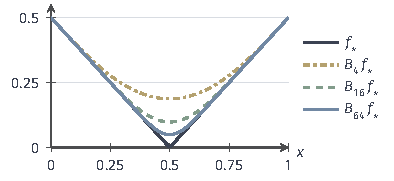
\includegraphics[width=66.7mm]{figures/02-abstract-mathematics/03-function-spaces/tikz/c6-bernstein-approx/figure.pdf}
  \caption{折线$f_*(x)=|x-1/2|$（黑）及其Bernstein多项式$B_4f_*$、$B_{16}f_*$、$B_{64}f_*$。每条曲线都是结点值的凸组合，位于$f_*$上方；一致误差都在$x=1/2$处取得，依次为$0.1875$、$0.0982$、$0.0497$，次数每增至四倍，误差约减半。}
  \label{fig:apx-bernstein-approx}
\end{figure}

凸组合只说明取值范围，还没有说明权重集中在哪些结点上。若权重主要落在离$x$较近的结点，$B_mf(x)$就主要由$f$在$x$附近的值决定。下面的矩恒等式把这个直觉写成精确的计算。

\begin{lemma}[Bernstein权重的矩]
\label{lem:apx-bernstein-moments}
对$0\le x\le1$和$m\ge1$，
\[
  \sum_{j=0}^m j\,w_{m,j}(x)=mx,\qquad
  \sum_{j=0}^m j(j-1)\,w_{m,j}(x)=m(m-1)x^2,
\]
从而
\begin{equation}
  \sum_{j=0}^m\Bigl(\frac jm-x\Bigr)^2w_{m,j}(x)=\frac{x(1-x)}m\le\frac1{4m}.
  \label{eq:apx-bernstein-variance}
\end{equation}
\end{lemma}

\begin{proof}
第一式利用$j\binom mj=m\binom{m-1}{j-1}$。$j=0$的项为零，把下标改为$k=j-1$，
\[
  \sum_{j=0}^m j\,w_{m,j}(x)
  =mx\sum_{k=0}^{m-1}\binom{m-1}{k}x^k(1-x)^{m-1-k}=mx,
\]
最后一步再次使用二项式定理。第二式同理利用$j(j-1)\binom mj=m(m-1)\binom{m-2}{j-2}$，把下标改为$k=j-2$即得；$m=1$时两边都为零。

对中心矩，把$(j/m-x)^2$展开，并用$j^2=j(j-1)+j$：
\[
  \sum_{j}\Bigl(\frac jm-x\Bigr)^2w_{m,j}
  =\frac{m(m-1)x^2+mx}{m^2}-2x\cdot\frac{mx}{m}+x^2
  =\frac{x(1-x)}m .
\]
最后由$x(1-x)\le1/4$得到上界$1/(4m)$。
\end{proof}

式~\eqref{eq:apx-bernstein-variance}说明，以$w_{m,j}(x)$为权重时，结点$j/m$与$x$的平均平方距离只有$x(1-x)/m$。若读者熟悉概率，这些权重正是二项分布$\mathrm{Bin}(m,x)$的概率，上述三式分别是总概率、均值与方差；证明只用到有限和，不依赖概率论。

\paragraph{近邻与远处的误差分解}

有了权重的集中性，就可以把误差分成两部分来控制：近邻结点上$f$的值接近$f(x)$，远处结点的总权重很小。

\begin{theorem}[Bernstein--Weierstrass逼近]
\label{thm:apx-bernstein}
设$f\in C([0,1])$。对每个$m\ge1$和每个$\delta>0$，
\begin{equation}
  \|B_mf-f\|_\infty\le\omega_f(\delta)+\frac{\|f\|_\infty}{2m\delta^2}.
  \label{eq:apx-bernstein-error}
\end{equation}
因此$\|B_mf-f\|_\infty\to0$（$m\to\infty$）。特别地，$[0,1]$上的多项式在$C([0,1])$中一致稠密。
\end{theorem}

\begin{proof}
固定$x\in[0,1]$。由权重和为一，误差可以写成
\[
  B_mf(x)-f(x)=\sum_{j=0}^m\Bigl[f\Bigl(\frac jm\Bigr)-f(x)\Bigr]w_{m,j}(x).
\]
按$|j/m-x|\le\delta$与$|j/m-x|>\delta$把结点分成近邻与远处两组。

近邻组中每个差值的绝对值不超过$\omega_f(\delta)$，而近邻权重之和不超过$1$，所以这一组的贡献至多为$\omega_f(\delta)$。

远处组中每个差值不超过$2\|f\|_\infty$。对远处的结点有$1<(j/m-x)^2/\delta^2$，于是由式~\eqref{eq:apx-bernstein-variance}，
\[
  \sum_{|j/m-x|>\delta}w_{m,j}(x)
  \le\frac1{\delta^2}\sum_{j=0}^m\Bigl(\frac jm-x\Bigr)^2w_{m,j}(x)
  \le\frac1{4m\delta^2},
\]
这一组的贡献至多为$2\|f\|_\infty/(4m\delta^2)$。两组相加后右端不依赖$x$，对$x$取上确界即得式~\eqref{eq:apx-bernstein-error}。

为了得到收敛，次序很重要。任给$\varepsilon>0$，先利用一致连续性选$\delta$使$\omega_f(\delta)<\varepsilon/2$；保持这个$\delta$不变，再取$m$足够大，使$\|f\|_\infty/(2m\delta^2)<\varepsilon/2$。若先固定$m$再缩小$\delta$，第二项会变大，论证不能成立。
\end{proof}

图~\ref{fig:apx-bernstein-weights}以$m=50$、$x=0.3$、$\delta=0.15$为例画出全部权重。蓝色的近邻结点占去权重$0.980$，黄色的远处结点只有$0.020$；矩估计给出的远处权重上界为$x(1-x)/(m\delta^2)=0.187$，再放大为$1/(4m\delta^2)=0.222$。上界相当保守，但它不依赖$x$，这正是全区间共用的误差界所需要的。

\begin{figure}[!htb]
  \centering
  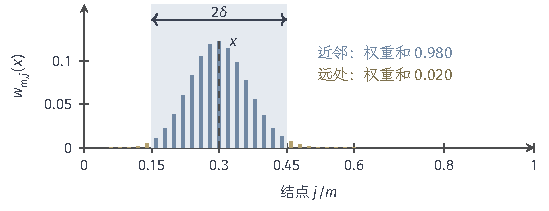
\includegraphics[width=93.0mm]{figures/02-abstract-mathematics/03-function-spaces/tikz/c6-bernstein-weights/figure.pdf}
  \caption{Bernstein权重的集中性：$m=50$、$x=0.3$时各结点$j/m$上的权重$w_{m,j}(x)$。蓝底为近邻窗口$|j/m-x|\le\delta=0.15$，窗口内权重和为$0.980$，窗口外（黄色）仅$0.020$。误差分解中，近邻部分由连续模$\omega_f(\delta)$控制，远处部分由二阶中心矩$x(1-x)/m$控制。}
  \label{fig:apx-bernstein-weights}
\end{figure}

\paragraph{折点目标与收敛速度}

定理~\ref{thm:apx-bernstein}保证$f_*$可以被多项式任意逼近，但任何一个多项式都不等于$f_*$：多项式处处可微，而$f_*$在$1/2$处的左右导数分别为$-1$和$1$。“可以任意逼近”与“能被某个有限次多项式精确表示”是两回事。

收敛有多快取决于目标的正则性。若$f$是$L$-Lipschitz的，可以不经过近远分解，直接用Cauchy--Schwarz不等式估计：
\[
  |B_mf(x)-f(x)|
  \le L\sum_{j}\Bigl|\frac jm-x\Bigr|w_{m,j}(x)
  \le L\Bigl(\sum_j\Bigl(\frac jm-x\Bigr)^2w_{m,j}(x)\Bigr)^{1/2}
  \le\frac{L}{2\sqrt m}.
\]
对$f_*$，$L=1$，这个界在$m=4,16,64$时分别为$0.25$、$0.125$、$0.0625$，实际误差$0.1875$、$0.0982$、$0.0497$与它同阶。对$\sqrt x$只有$|f(s)-f(t)|\le|s-t|^{1/2}$，同样的论证（先对$|j/m-x|^{1/2}$用Cauchy--Schwarz）只给出$(4m)^{-1/4}$。条件越弱，这个构造能保证的速率越慢。

Bernstein多项式也不是相应次数下最好的多项式。由引理~\ref{lem:apx-bernstein-moments}，
\[
  B_m(x^2)=\frac{m(m-1)x^2+mx}{m^2}=x^2+\frac{x(1-x)}m,
\]
所以对$x^2$本身，误差恰为$1/(4m)$，而$x^2$只是一个二次多项式。这个构造的价值在于每一步都可以验证，并给出所有连续函数共同的收敛机制；最佳逼近的误差需要另外研究。

\paragraph{Stone--Weierstrass定理}

回看定理~\ref{thm:apx-bernstein}的结论：$[0,1]$上的多项式在一致范数下稠密。把多项式换成其他函数族、把区间换成其他紧集时，哪些性质仍然是关键？多项式族对加法、数乘和乘法封闭，含有常数，而且函数$x$能区分任意两个不同的点。下面的定理说明这几条已经足够。

设$K$是非空紧度量空间，$C(K)$为$K$上全体实值连续函数，配备一致范数。若子空间$\mathcal A\subseteq C(K)$对逐点乘法封闭，就称它是\term{子代数}（subalgebra）；若对任意$x\ne y$都有$h\in\mathcal A$使$h(x)\ne h(y)$，就称$\mathcal A$\term{分离点}（separates points）。

\begin{theorem}[Stone--Weierstrass定理]
\label{thm:apx-stone-weierstrass}
设$K$是非空紧度量空间，$\mathcal A\subseteq C(K)$是含有常数函数且分离点的子代数，则$\mathcal A$在$C(K)$中按一致范数稠密：对每个$f\in C(K)$和$\varepsilon>0$，存在$h\in\mathcal A$使$\|f-h\|_\infty<\varepsilon$。
\end{theorem}

这一结论由Stone对Weierstrass多项式逼近定理的推广给出\scite{stone1948generalized}。它立即覆盖多变量的情形：在紧集$K\subset\mathbb R^d$上，$d$元多项式组成含常数的子代数，坐标函数分离点，因此多元多项式在$C(K)$中稠密。另一个例子是单位圆周：把$[0,2\pi]$的两端看成同一点，三角多项式$\sum_{k=0}^n(a_k\cos kt+b_k\sin kt)$对乘法封闭（由积化和差），含有常数，$\cos t$与$\sin t$合起来分离圆周上的点，因此在圆周上的连续函数中稠密。

两个条件各自不可缺少。在$[-1,1]$上，偶多项式组成含常数的子代数，但对每个偶多项式都有$p(x)=p(-x)$，它不能分离$x$与$-x$；一致极限仍是偶函数，因此奇函数$x$不在闭包中。在$[0,1]$上，满足$p(0)=0$的多项式组成分离点的子代数，但不含常数；一致极限都在$0$处取零，所以常函数$1$不在闭包中。

\begin{proof}[补充阅读：证明思路]
记$\overline{\mathcal A}$为一致闭包，它仍是含常数的子代数。第一步，若$h\in\overline{\mathcal A}$，则$|h|\in\overline{\mathcal A}$：在$[-\|h\|_\infty,\|h\|_\infty]$上用多项式$p$一致逼近$|t|$（定理~\ref{thm:apx-bernstein}经线性变量代换），$p\circ h$属于$\overline{\mathcal A}$且一致接近$|h|$。由$\max\{g,h\}=(g+h+|g-h|)/2$和$\min\{g,h\}=(g+h-|g-h|)/2$，$\overline{\mathcal A}$对有限个函数取最大、最小封闭。第二步，由分离点和常数，对任意$x\ne y$和实数$a,b$，存在$h\in\mathcal A$满足$h(x)=a$、$h(y)=b$：取$u$使$u(x)\ne u(y)$，令$h=a+(b-a)(u-u(x))/(u(y)-u(x))$。第三步，固定$f$、$\varepsilon$和$x$，对每个$y$取$h_y$使$h_y(x)=f(x)$、$h_y(y)=f(y)$；集合$\{z:h_y(z)<f(z)+\varepsilon\}$是开集并覆盖$K$，由紧性取有限个，令$g_x=\min h_{y_i}$，则$g_x<f+\varepsilon$且$g_x(x)=f(x)$。再对开集$\{z:g_x(z)>f(z)-\varepsilon\}$用一次紧性，取有限个$g_{x_k}$的最大值，即得$\overline{\mathcal A}$中与$f$一致误差小于$\varepsilon$的函数。
\end{proof}

\paragraph{稠密性与误差速率}

Stone--Weierstrass定理只回答“能否任意逼近”，不提供任何速率：它没有说明达到精度$\varepsilon$需要多少项，证明中的紧性步骤也不给出项数。定理~\ref{thm:apx-bernstein}之所以能给出速率，是因为对目标另加了连续模或Lipschitz常数等定量条件。要比较不同生成单元的效率，必须先固定这样一个函数类；第~\ref{sec:apx-function-classes}节将把“固定一个函数类”本身作为研究对象。

\subsection{样条逼近}
\label{sec:apx-splines}

多项式是全局的：改变一个系数，整个区间上的函数值都会改变，Bernstein权重也在整个$(0,1)$上非零。另一种思路是把区间切成小段，每段只用低次多项式，段与段之间按一定光滑性衔接。这类分段多项式称为\term{样条}（spline），分段的位置称为\term{结点}（knot）。本小节从最简单的连续分段直线开始。

\paragraph{线性插值与连续模界}

固定结点$0=t_0<t_1<\cdots<t_N=1$，记最大间距$h=\max_i(t_{i+1}-t_i)$。对$x\in[t_i,t_{i+1}]$，令
\begin{equation}
  S_hf(x)=(1-s)f(t_i)+s\,f(t_{i+1}),\qquad s=\frac{x-t_i}{t_{i+1}-t_i}\in[0,1].
  \label{eq:apx-linear-interpolant}
\end{equation}
相邻两段在公共结点取同一个值，所以$S_hf$是经过全部结点值的连续折线，称为$f$的线性插值。全体在每段上为一次函数的连续函数组成\term{线性样条}（linear spline）空间，它是$N+1$维的线性空间；$S_h$则是从结点值产生其中一个元素的操作。图~\ref{fig:apx-spline-hat}(a)画出一个光滑函数在七个等距结点上的线性插值。

\begin{theorem}[线性插值的误差]
\label{thm:apx-linear-interpolation}
在上述记号下，若$f\in C([0,1])$，则
\begin{equation}
  \|f-S_hf\|_\infty\le\omega_f(h).
  \label{eq:apx-spline-modulus}
\end{equation}
若进一步$f\in C^2([0,1])$，则
\begin{equation}
  \|f-S_hf\|_\infty\le\frac{h^2}{8}\|f''\|_\infty .
  \label{eq:apx-spline-quadratic}
\end{equation}
\end{theorem}

\begin{proof}
先证连续模界。在单元$[t_i,t_{i+1}]$上，利用$(1-s)+s=1$，
\[
  f(x)-S_hf(x)=(1-s)\bigl(f(x)-f(t_i)\bigr)+s\bigl(f(x)-f(t_{i+1})\bigr).
\]
$x$到两个端点的距离都不超过$h$，所以两个差值都不超过$\omega_f(h)$，凸组合也不超过$\omega_f(h)$。对所有单元取上确界即得式~\eqref{eq:apx-spline-modulus}。

再证二阶界。固定单元和其中一点$x\in(t_i,t_{i+1})$，令$g=f-S_hf$，它在两端为零。取
\[
  \lambda=\frac{g(x)}{(x-t_i)(x-t_{i+1})},\qquad
  G(u)=g(u)-\lambda(u-t_i)(u-t_{i+1}),
\]
则$G$在$t_i$、$x$、$t_{i+1}$三点为零。两次使用Rolle定理，存在$\xi\in(t_i,t_{i+1})$使$G''(\xi)=0$。由于$S_hf$在单元内是一次函数，$G''(\xi)=f''(\xi)-2\lambda$，故$\lambda=f''(\xi)/2$，即
\[
  f(x)-S_hf(x)=\frac{f''(\xi)}2(x-t_i)(x-t_{i+1}).
\]
在单元上$|(x-t_i)(x-t_{i+1})|\le(t_{i+1}-t_i)^2/4\le h^2/4$，代入即得式~\eqref{eq:apx-spline-quadratic}。
\end{proof}

两个界依据不同。连续模界只用了凸组合，对任何连续目标成立，并且不要求结点等距：只要一列网格的最大间距$h\to0$，插值就一致收敛到$f$。二阶界多用了$f''$的有界性，换来$h^2$的速率；Rolle定理与插值余项可参考\BookChapterRef{chap:univariate-differentiation}{卷一“一元函数的微分”章}。

二阶界中的常数$1/8$不能改进。取$f(x)=x^2$，只用两个结点$0$和$1$，则$S_hf(x)=x$，误差$x-x^2$在$x=1/2$处取最大值$1/4$；此时$h=1$、$\|f''\|_\infty=2$，右端$h^2\|f''\|_\infty/8=1/4$，等号成立。

\paragraph{额外光滑性带来的速率}

二阶速率所用的光滑性不能省略。取等距结点$t_i=i/N$，$N$为奇数，此时$1/2$不是结点，而落在单元$[(N-1)/(2N),(N+1)/(2N)]$的中点。$f_*$在这个单元的两个端点取值都是$h/2$，插值在单元内恒为$h/2$，而$f_*(1/2)=0$；其余单元上$f_*$本身就是直线，插值没有误差。因此$\|f_*-S_hf_*\|_\infty=h/2$，只按一阶下降，这与$\omega_{f_*}(h)=h$的界同阶。

图~\ref{fig:apx-spline-rates}在对数坐标中比较两种目标。光滑函数$\sin(\pi x)$的实测误差几乎落在二阶界$\pi^2h^2/8$上，斜率为$2$；$f_*$的误差落在直线$h/2$上，斜率为$1$。网格宽度控制的是表示的分辨率，同一分辨率下能达到的精度取决于目标的光滑性。

\begin{figure}[!htb]
  \centering
  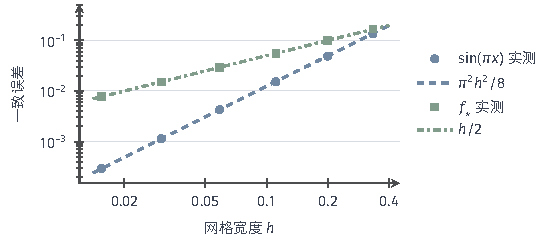
\includegraphics[width=93.4mm]{figures/02-abstract-mathematics/03-function-spaces/tikz/c6-spline-rates/figure.pdf}
  \caption{等距线性插值的一致误差与网格宽度$h=1/N$（$N=3,5,\ldots,65$为奇数，$1/2$不是结点），双对数坐标。光滑目标$\sin(\pi x)$的误差（圆点）贴近二阶界$\pi^2h^2/8$；折线$f_*$的误差（方块）恰为$h/2$，只按一阶下降。}
  \label{fig:apx-spline-rates}
\end{figure}

\paragraph{帽形基与局部修改}

线性插值可以改写成固定基函数的线性组合。对每个结点$t_i$，令$\varphi_i$为在$t_i$处取$1$、在其余结点处取$0$的线性样条；它在$[t_{i-1},t_{i+1}]$上呈三角形，在别处为零，称为\term{帽形函数}（hat function）。于是
\[
  S_hf=\sum_{i=0}^{N}f(t_i)\varphi_i,\qquad \sum_{i=0}^N\varphi_i\equiv1 .
\]
系数恰好是结点值，基函数非负且和为一，这正是式~\eqref{eq:apx-linear-interpolant}中凸组合的来源。

若结点包含$1/2$，例如取$t_0=0$、$t_1=1/2$、$t_2=1$，则$f_*$在每段上都是直线，
\[
  f_*=\tfrac12\varphi_0+0\cdot\varphi_1+\tfrac12\varphi_2 ,
\]
三个系数就精确表示了它。这比任何次数的多项式都节省，原因在于结点恰好放在折点上；同一组结点并不能精确表示任意连续目标。

帽形基的支撑只覆盖相邻两段，因此修改一个结点值只影响局部。图~\ref{fig:apx-spline-hat}(b)把$t_3=1/2$处的值由$0.5$改为$0.8$，插值只在$[t_2,t_4]=[1/3,2/3]$上改变。这里有两个不同来源的性质：局部性来自基函数的支撑，误差界来自凸组合；后面换用其他基时，需要分别重新检查。

\begin{figure}[!htb]
  \centering
  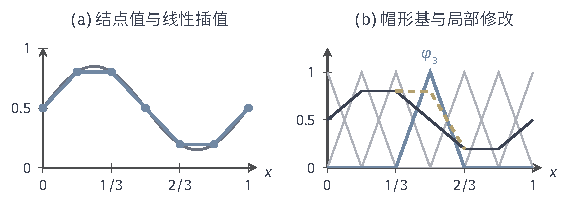
\includegraphics[width=96.2mm]{figures/02-abstract-mathematics/03-function-spaces/tikz/c6-spline-hat/figure.pdf}
  \caption{线性样条与帽形基，结点$t_i=i/6$。(a)~目标$0.5+0.35\sin(2\pi x)$（灰）及其线性插值（蓝折线），圆点为结点值。(b)~七个帽形函数（细灰），其中$\varphi_3$加粗；黑色折线为(a)中的插值，把$t_3$处的结点值改为$0.8$后得到黄色虚线，变化只发生在$\varphi_3$的支撑$[1/3,2/3]$上。}
  \label{fig:apx-spline-hat}
\end{figure}

\paragraph{高次样条与系数恢复}

把每段的一次函数换成$k$次多项式，并要求在内部结点处$k-1$阶导数连续，就得到$k$次样条。$N$段各有$k+1$个系数，每个内部结点施加$k$个衔接条件，空间维数为$(k+1)N-k(N-1)=N+k$。常用的三次样条维数为$N+3$，而结点值只提供$N+1$个条件，还需补充两个端点条件，插值才唯一。

更高的次数和衔接阶带来更光滑的近似，代价是系数与结点值不再直接对应。以等距结点上的三次B样条$\beta_3$为例（$\beta_3(0)=2/3$，$\beta_3(\pm1)=1/6$，在$|s|\ge2$处为零），若$S(x)=\sum_jc_j\beta_3(x-j)$，则在整数结点处
\[
  S(i)=\frac{c_{i-1}+4c_i+c_{i+1}}6 .
\]
要让$S$经过给定的结点值，必须先解这个线性方程组恢复系数；直接把结点值当系数，得到的是相邻值的加权平均。因此要分清三件事：样条空间是哪个候选集合，插值条件从中挑出哪个元素，系数又如何从样本求出。图像重采样中的插值核、预滤波和边界延拓属于信号处理的具体问题，可参考\BookChapterRef{chap:signal-analysis}{卷三“信号”章}。

\subsection{核截面逼近}
\label{sec:apx-kernel-sections}

第~\ref{chap:rkhs}章从半正定核$K$构造了再生核Hilbert空间$H_K$，并证明核截面$K_x=K(\cdot,x)$的有限线性组合在$H_K$中按核范数稠密（第~\ref{sec:rkhs-from-kernel}节）。本小节把核截面当作生成单元，问：在$H_K$之外，有限核和能否逼近更一般的连续目标？

\paragraph{核空间内与核空间外}

先说明核范数下的逼近在什么意义上已经是一致逼近。由再生关系$f(x)=\langle f,K_x\rangle_{H_K}$和Cauchy--Schwarz不等式，$|f(x)|\le\sqrt{K(x,x)}\,\|f\|_{H_K}$（第~\ref{sec:rkhs-kernel-properties}节）。若$\sup_xK(x,x)<\infty$，则$\|f\|_\infty\le\sup_x\sqrt{K(x,x)}\,\|f\|_{H_K}$，核范数下的逼近自动是一致逼近。

本小节固定$[0,1]$上宽度为$\sigma>0$的高斯核
\[
  K_\sigma(x,c)=\exp\Bigl(-\frac{(x-c)^2}{2\sigma^2}\Bigr),
\]
它满足$K_\sigma(x,x)=1$，所以$\|f\|_\infty\le\|f\|_{H_K}$。问题在于$f_*$不属于这个$H_K$。原因是$H_K$中的函数都可微。由再生关系，两个差商$(K_{x+t}-K_x)/t$与$(K_{x+t'}-K_x)/t'$的内积等于
\[
  \frac{K(x+t,x+t')-K(x+t,x)-K(x,x+t')+K(x,x)}{tt'},
\]
$K_\sigma$二阶连续可微，$t,t'\to0$时它趋于$\partial_1\partial_2K(x,x)$。于是差商之差的范数平方$\|(K_{x+t}-K_x)/t-(K_{x+t'}-K_x)/t'\|_{H_K}^2$趋于零，差商在完备空间$H_K$中收敛到某个$D_x$；于是对$f\in H_K$，
\[
  \frac{f(x+t)-f(x)}t=\Bigl\langle f,\frac{K_{x+t}-K_x}t\Bigr\rangle_{H_K}\to\langle f,D_x\rangle_{H_K},
\]
$f$在$x$处可导。$f_*$在$1/2$处不可导，所以$f_*\notin H_K$，第~\ref{chap:rkhs}章的稠密性结论不能直接用于它。

\paragraph{中心差分与加权多项式}

证明的思路是借助多项式。先固定中心$c_0=1/2$，令$w(x)=K_\sigma(x,c_0)$。对中心求导，$\partial_cK_\sigma(x,c)=(x-c)K_\sigma(x,c)/\sigma^2$，每求一次导就多出一个关于$x$的一次因子。由归纳法，
\begin{equation}
  \partial_c^jK_\sigma(x,c_0)=w(x)P_j(x),
  \label{eq:apx-gaussian-derivative}
\end{equation}
其中$P_j$是$j$次多项式，最高次项系数为$\sigma^{-2j}$。归纳步骤是：对$K_\sigma(x,c)Q(x-c)$再关于$c$求导，得到$K_\sigma(x,c)\bigl[(x-c)Q(x-c)/\sigma^2-Q'(x-c)\bigr]$，第一项把次数提高一次并把首项系数乘以$\sigma^{-2}$，第二项次数更低。

导数本身还不是有限核和，需要用差分代替。对固定的$j$和步长$t>0$，中心$j$阶前向差分
\begin{equation}
  D_t^{(j)}(x)=t^{-j}\sum_{\ell=0}^{j}(-1)^{j-\ell}\binom j\ell K_\sigma(x,c_0+\ell t)
  \label{eq:apx-center-difference}
\end{equation}
是$j+1$个核截面的线性组合。反复使用微积分基本定理，可以把它写成导数的平均：
\[
  D_t^{(j)}(x)=t^{-j}\int_0^t\!\!\cdots\!\int_0^t\partial_c^jK_\sigma(x,c_0+u_1+\cdots+u_j)\,\mathrm du_1\cdots\mathrm du_j .
\]
积分中的中心都落在$[c_0,c_0+jt]$内。$\partial_c^jK_\sigma$在紧矩形$[0,1]\times[c_0,c_0+1]$上一致连续，所以
\[
  \begin{aligned}
  \sup_{x\in[0,1]}\bigl|D_t^{(j)}(x)-w(x)P_j(x)\bigr|
  &\le\sup_{x\in[0,1],\ 0\le u\le jt}\bigl|\partial_c^jK_\sigma(x,c_0+u)-\partial_c^jK_\sigma(x,c_0)\bigr|\\
  &\to0\qquad(t\downarrow0).
  \end{aligned}
\]
一致性来自这里的二元一致连续，逐点求导本身只给出每个$x$处的收敛。图~\ref{fig:apx-gaussian-sections}(b)画出$j=1$的情形：$t=0.1$时差分与导数的一致偏差为$2.14$，$t=0.02$时降为$0.44$。

\paragraph{高斯核截面的一致稠密性}

有了每个$wP_j$都能由有限核和一致逼近，剩下的工作是把任意连续目标化成$w$乘一个多项式。

\begin{theorem}[固定宽度高斯核截面的一致稠密性]
\label{thm:apx-gaussian-dense}
固定$\sigma>0$。全体有限和$\sum_{\ell=1}^{M}a_\ell K_\sigma(\cdot,c_\ell)$（$M\in\mathbb N$、$a_\ell\in\mathbb R$、$c_\ell\in\mathbb R$均可随目标和精度变化）在$C([0,1])$中按一致范数稠密。
\end{theorem}

\begin{proof}
设$f\in C([0,1])$，$\varepsilon>0$。

第一步，把目标化成加权多项式。$w$在$[0,1]$上连续且有正下界，所以$f/w\in C([0,1])$。由定理~\ref{thm:apx-bernstein}，存在多项式$P$使$\|f/w-P\|_\infty<\varepsilon/2$；由$0<w\le1$，得$\|f-wP\|_\infty<\varepsilon/2$。

第二步，把$P$写成$P_0,\ldots,P_n$的组合，其中$n=\deg P$。$P_j$的首项系数$\sigma^{-2j}\ne0$，所以从$1,x,\ldots,x^n$到$P_0,\ldots,P_n$的系数矩阵是对角元非零的三角矩阵，可逆。因此$P=\sum_{j=0}^nb_jP_j$，$wP=\sum_jb_jwP_j$。

第三步，对每个$j$用差分代替$wP_j$。由上一段的一致收敛，可选步长$t_j$使$\|D_{t_j}^{(j)}-wP_j\|_\infty<\varepsilon/\bigl(2(n+1)(|b_j|+1)\bigr)$。于是$g=\sum_jb_jD_{t_j}^{(j)}$是有限个高斯核截面的线性组合，且
\[
  \|f-g\|_\infty\le\|f-wP\|_\infty+\sum_{j=0}^n|b_j|\,\|wP_j-D_{t_j}^{(j)}\|_\infty<\varepsilon.
\]
\end{proof}

图~\ref{fig:apx-gaussian-sections}(a)取$\sigma=0.15$，在$M$个等距中心处插值$f_*$：$M=5$时一致误差为$0.061$，$M=9$时为$0.024$。这只是一种具体的选系数方式，并不是定理证明中的构造。

\begin{figure}[!htb]
  \centering
  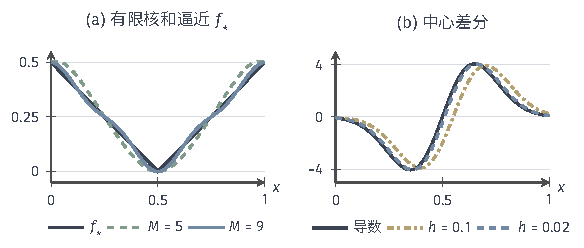
\includegraphics[width=98.9mm]{figures/02-abstract-mathematics/03-function-spaces/tikz/c6-gaussian-sections/figure.pdf}
  \caption{固定宽度$\sigma=0.15$的高斯核截面。(a)~在等距中心$c_\ell=(\ell-1)/(M-1)$处插值$f_*$的有限核和，$M=5$（虚线）与$M=9$（实线），一致误差分别为$0.061$与$0.024$。(b)~中心差分$(K_\sigma(x,\frac12+t)-K_\sigma(x,\frac12))/t$随$t$减小一致逼近导数$(x-\frac12)K_\sigma(x,\frac12)/\sigma^2$，这是一个加权一次多项式。}
  \label{fig:apx-gaussian-sections}
\end{figure}

\paragraph{两种稠密性与结论的条件}

现在可以区分两个命题。第~\ref{chap:rkhs}章的结论是：核截面的有限和在$H_K$中按核范数稠密，它只涉及$H_K$内部的函数。定理~\ref{thm:apx-gaussian-dense}则是：有限核和在$C([0,1])$中按一致范数稠密，它涉及$H_K$之外的目标，例如$f_*$。紧度量空间$X$上的连续核若使$H_K$在$C(X)$中稠密，就称为\term{通用核}（universal kernel）。由于$\|g\|_\infty\le\sup_x\sqrt{K(x,x)}\,\|g\|_{H_K}$，$H_K$中每个元素都能被有限核和一致逼近，所以“$H_K$在$C(X)$中稠密”与“有限核和在$C(X)$中稠密”是同一回事。Steinwart证明了高斯核在$\mathbb R^d$的任意紧子集上都是通用核\cite{steinwart2001kernel}；上面给出的是一维区间上的一条具体证明路线。

定理的条件同样需要逐条读清。

第一，中心、项数和系数都允许随目标与精度变化。若只允许一组预先固定的有限中心，得到的是$C([0,1])$中的有限维子空间；有限维子空间是闭的且不是全空间，不可能稠密。

第二，定理没有对系数或核范数设统一预算。第~\ref{sec:apx-arzela-ascoli}节将证明，核范数不超过$R$的函数组成$C([0,1])$中的紧集，因而是闭集；它只含$H_K$中的函数，所以不含$f_*$，$f_*$到它的一致距离为正。由此，逼近$f_*$的有限核和的核范数必然随精度趋于无穷。

第三，存在性证明不提供数值稳定的选系数方法。差分中出现因子$t^{-j}$，系数会随精度变大；朴素插值也有同样的问题：$\sigma=0.15$时，$M=13$个等距中心的插值误差为$0.023$，最大系数约为$415$；$M=17$时最大系数约为$1.06\times10^6$，误差反而升到$0.097$。如何在给定数据和惩罚下稳定地确定系数，属于后续优化与拟合问题。

\subsection{神经网络逼近}
\label{sec:apx-neural}

神经单元先对输入作仿射变换，再送入一个固定的一元函数，即激活函数；网络的输出是若干单元的线性组合。本小节从一维的分段线性构造开始，把它和样条联系起来，再陈述一般的通用逼近定理。

\paragraph{ReLU单元与折点目标}

\term{整流线性单元}（rectified linear unit，ReLU）使用激活函数$\rho(s)=\max\{s,0\}$。一个单元$x\mapsto a\rho(wx+b)$在$x=-b/w$处折一次，一侧为零，另一侧为斜率$aw$的直线。对贯穿目标，直接验证
\[
  f_*(x)=\rho\Bigl(x-\frac12\Bigr)+\rho\Bigl(\frac12-x\Bigr):
\]
当$x\ge1/2$时第一项为$x-1/2$、第二项为零；当$x\le1/2$时第一项为零、第二项为$1/2-x$。两个单元的输入权重符号相反，偏置都把折点放在$1/2$，输出直接相加，见图~\ref{fig:apx-relu-units}(a)。这个表示由两侧的计算验证，与训练过程无关。

\paragraph{线性样条的ReLU分解}

每个ReLU单元贡献一个折点，这提示连续折线都可以用ReLU单元写出。设连续函数$f$在$[t_0,t_N]$上以$t_0<t_1<\cdots<t_N$为结点分段线性，第$k$段$[t_k,t_{k+1}]$上的斜率为$s_k$。则
\begin{equation}
  f(x)=f(t_0)+s_0(x-t_0)+\sum_{k=1}^{N-1}(s_k-s_{k-1})\rho(x-t_k),\qquad x\in[t_0,t_N].
  \label{eq:apx-relu-spline}
\end{equation}
验证只需比较两侧：右端在$x=t_0$处等于$f(t_0)$，是连续折线；在第$k$段内部，$\rho(x-t_1),\ldots,\rho(x-t_k)$都已进入线性部分，斜率为$s_0+\sum_{i=1}^k(s_i-s_{i-1})=s_k$，与$f$相同。两个连续函数在起点相等且每段斜率相同，所以处处相等。每个单元只在自己的结点之后改变斜率，图~\ref{fig:apx-relu-units}(b)画出了逐项相加的部分和。

在$[0,1]$上$t_0=0$时，$s_0x=s_0\rho(x)$，常数项可以作为输出偏置，因此式~\eqref{eq:apx-relu-spline}恰是一个有$N$个隐藏单元的单隐藏层ReLU网络；在一般区间上可用$x=\rho(x)-\rho(-x)$补出线性项。结合定理~\ref{thm:apx-linear-interpolation}，取等距结点$t_k=k/N$并对$f\in C([0,1])$作线性插值，就得到一个$N$单元网络$g_N$，满足
\[
  \|f-g_N\|_\infty\le\omega_f(1/N).
\]
这是一维ReLU网络通用逼近的构造性证明，同时给出速率：对$L$-Lipschitz目标，误差不超过$L/N$。

\begin{figure}[!htb]
  \centering
  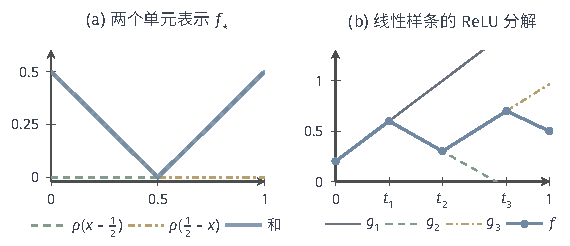
\includegraphics[width=96.6mm]{figures/02-abstract-mathematics/03-function-spaces/tikz/c6-relu-units/figure.pdf}
  \caption{ReLU单元的有限组合。(a)~$\rho(x-\frac12)$与$\rho(\frac12-x)$之和恰为$f_*$。(b)~结点$0,t_1,t_2,t_3,1=0,0.25,0.5,0.8,1$、结点值$0.2,0.6,0.3,0.7,0.5$的线性样条$f$（蓝），按式~\eqref{eq:apx-relu-spline}写成$0.2+1.6\rho(x)-2.8\rho(x-0.25)+\frac{38}{15}\rho(x-0.5)-\frac73\rho(x-0.8)$；细线$g_1,g_2,g_3$依次是前一、二、三个单元的部分和，每加一个单元就在对应结点处改变斜率。}
  \label{fig:apx-relu-units}
\end{figure}

\paragraph{单隐藏层通用逼近定理}

一维构造依赖分段线性的特殊结构。对多维输入和一般激活函数，需要下面的存在定理。

\begin{theorem}[单隐藏层网络的通用逼近]
\label{thm:apx-universal-approximation}
设$X\subset\mathbb R^d$是非空紧集，激活函数$\sigma:\mathbb R\to\mathbb R$连续且不是多项式。则形如
\begin{equation}
  g(\bm x)=\sum_{j=1}^{M}a_j\,\sigma(\bm w_j^{\top}\bm x+b_j),
  \qquad M\in\mathbb N,\ a_j,b_j\in\mathbb R,\ \bm w_j\in\mathbb R^d
  \label{eq:apx-one-hidden-layer}
\end{equation}
的函数全体在$C(X)$中按一致范数稠密。
\end{theorem}

这一形式的结论由Leshno、Lin、Pinkus与Schocken证明\cite{leshno1993approximation}，他们的结果对更广的局部有界、分段连续激活也成立；此前Cybenko对S型激活给出了同类结论\scite{cybenko1989approximation}。这里只陈述并使用连续激活的情形，证明从略。在式~\eqref{eq:apx-one-hidden-layer}外再加一个输出偏置，不改变结论。

定理的条件都可以用例子检查。Sigmoid函数$1/(1+e^{-s})$、$\tanh s$和ReLU都连续且不是多项式，所以都满足条件；定理不要求激活处处可微。

多项式激活必须排除。若$\sigma$是$r$次多项式，则$\sigma(\bm w^{\top}\bm x+b)$是$\bm x$的至多$r$次多项式，无论$M$多大，$g$都落在“$d$元至多$r$次多项式”这个有限维子空间中。若$X$含有内点，函数$x_1^{r+1}$不在这个子空间中；有限维子空间是闭的，所以$x_1^{r+1}$与它的一致距离为正。增加宽度不能增加可表达的次数，“使用了非线性函数”不能代替“非多项式”这一条件。

偏置也不能省略。在$[0,1]$上取ReLU且令所有$b_j=0$，则$\rho(w_jx)$在$w_j>0$时等于$w_jx$，在$w_j\le0$时恒为零，所有组合都形如$cx$。这样的函数在$0$处为零，无法逼近常函数$1$。

\paragraph{表示能力之外的问题}

通用逼近定理断言“存在”一组参数，它不回答以下几个问题，每个都需要单独的条件和论证。

参数不可识别。同一个函数有许多参数表示：交换隐藏单元的次序不改变输出；ReLU的正齐次性给出$a\rho(wx+b)=(a/\lambda)\rho(\lambda wx+\lambda b)$（$\lambda>0$）；在$[0,1]$上还有$f_*(x)=2\rho(x-\frac12)-\rho(x)+\frac12$，它与前面的两单元表示使用不同的单元。因此不能由函数反推出唯一的参数。

寻找参数与推广到新样本是另外的问题。定理不说明梯度方法能否找到逼近参数，也不说明由有限样本训练出的网络在新输入上误差小；相应的分析可参考\BookChapterRef{chap:feedforward-networks}{卷八“前馈神经网络”章}和\BookChapterRef{chap:deep-learning-theory}{卷六“深度学习的可学习性”章}。

评价范数也要说明。若输入服从$X$上的概率测度$\mu$，则$\|f-g\|_{L^2(\mu)}\le\|f-g\|_\infty$，一致逼近自动给出平均意义下的逼近；反方向不成立，一个只在小区域上很高的尖峰可以使$L^2(\mu)$误差很小而一致误差很大。向量值目标可以逐坐标逼近，再把各坐标的隐藏单元并列放进同一隐藏层。

% 第8章第2节：多变量函数的组合表示（张量积函数空间、低秩分离表示）。

\section{多变量函数的组合表示}
\label{sec:apx-multivariate}

上一节讨论的是选择什么生成单元。目标有多个变量时，还要决定怎样由单变量的函数组成多变量的函数。本节把变量分成两组$x$与$y$（每组本身也可以是向量），研究乘积$u(x)v(y)$的有限和。张量积空间描述全部这样的组合能张成什么；低秩表示则在这个空间中只使用少数几个乘积项。两者可以使用同样的单变量生成函数，区别在于用了多少个乘积方向。

记$(u\otimes v)(x,y)=u(x)v(y)$，称为$u$与$v$的乘积函数，也称为\term{张量积}（tensor product）。

\subsection{张量积函数空间}
\label{sec:apx-tensor-product}

\paragraph{乘积函数与系数矩阵}

固定$x$方向的函数$\varphi_1,\ldots,\varphi_m$和$y$方向的函数$\psi_1,\ldots,\psi_n$，并设每组都线性无关。所有乘积$\varphi_i\otimes\psi_k$的线性组合可以写成
\begin{equation}
  F(x,y)=\sum_{i=1}^m\sum_{k=1}^n c_{i,k}\varphi_i(x)\psi_k(y)=\bm\varphi(x)^{\top}\bm C\,\bm\psi(y),
  \label{eq:apx-coefficient-matrix}
\end{equation}
其中$\bm\varphi(x)=(\varphi_1(x),\ldots,\varphi_m(x))^{\top}$，$\bm\psi(y)$类似，$\bm C=[c_{i,k}]\in\mathbb R^{m\times n}$是系数矩阵。把$\bm C$按列拉直成$\operatorname{vec}(\bm C)\in\mathbb R^{mn}$，则$F(x,y)=(\bm\psi(y)\otimes\bm\varphi(x))^{\top}\operatorname{vec}(\bm C)$，这里的$\otimes$是Kronecker积；有限维的张量积与Kronecker积可参考\BookChapterRef{chap:linear-operations}{卷一“向量、矩阵与张量的运算”章}。

系数矩阵由$F$唯一确定。若$\sum_{i,k}c_{i,k}\varphi_i(x)\psi_k(y)\equiv0$，固定$y$后，由$\varphi_i$线性无关得$\sum_kc_{i,k}\psi_k(y)=0$对每个$i$和每个$y$成立，再由$\psi_k$线性无关得全部$c_{i,k}=0$。因此$mn$个乘积函数线性无关，组成的空间维数为$mn$。

矩阵的秩对应最少的乘积项数。若在这两个子空间中$F=\sum_{j=1}^ru_j\otimes v_j$，把$u_j=\bm\varphi^{\top}\bm a_j$、$v_j=\bm\psi^{\top}\bm b_j$代入，由系数唯一性得$\bm C=\sum_{j=1}^r\bm a_j\bm b_j^{\top}$，所以$r\ge\operatorname{rank}\bm C$；反之，$\bm C$的秩分解直接给出$\operatorname{rank}\bm C$项的表示。例如$F(x,y)=x+y=x\cdot1+1\cdot y$，在基$\{1,x\}$与$\{1,y\}$下系数矩阵为$\left[\begin{smallmatrix}0&1\\1&0\end{smallmatrix}\right]$，秩为$2$，所以$x+y$不是单个乘积函数；而$e^{x+y}=e^xe^y$只需一项。

\paragraph{乘积测度下的内积}

要讨论$L^2$误差，需要知道乘积函数的内积怎样计算。设$(X,\mu)$与$(Y,\nu)$是有限测度空间，$\mu\otimes\nu$为乘积测度。对实值$u,u'\in L^2(\mu)$与$v,v'\in L^2(\nu)$，由Cauchy--Schwarz不等式，$uu'\in L^1(\mu)$且$vv'\in L^1(\nu)$，于是$(u\otimes v)(u'\otimes v')$在$\mu\otimes\nu$下可积，由第~\ref{chap:measure-spaces}章中$\sigma$有限乘积测度的Fubini定理，
\begin{equation}
  \langle u\otimes v,u'\otimes v'\rangle_{L^2(\mu\otimes\nu)}
  =\int_X u u'\,\mathrm d\mu\int_Y v v'\,\mathrm d\nu
  =\langle u,u'\rangle_{L^2(\mu)}\langle v,v'\rangle_{L^2(\nu)} .
  \label{eq:apx-product-inner}
\end{equation}
特别地$\|u\otimes v\|=\|u\|\,\|v\|$，乘积函数属于$L^2(\mu\otimes\nu)$。乘积的内积分解为两个因子内积的乘积，这是下面构造正交基的依据。

\paragraph{正交基的乘积}

由式~\eqref{eq:apx-product-inner}，两组标准正交系的乘积仍是标准正交系。下面的定理说明，在可分情形它还是完备的。

\begin{theorem}[乘积正交基]
\label{thm:apx-product-basis}
设$(X,\mu)$与$(Y,\nu)$是有限测度空间，实空间$L^2(\mu)$与$L^2(\nu)$可分，分别有标准正交基$\{e_i\}_{i\ge1}$与$\{f_k\}_{k\ge1}$。则$\{e_i\otimes f_k\}_{i,k\ge1}$是$L^2(\mu\otimes\nu)$的标准正交基。
\end{theorem}

\begin{proof}
标准正交性由式~\eqref{eq:apx-product-inner}直接得到，只需证明完备：若$F\in L^2(\mu\otimes\nu)$与所有$e_i\otimes f_k$正交，则$F=0$。

由Tonelli定理，$\int_X\bigl(\int_Y|F(x,y)|^2\mathrm d\nu\bigr)\mathrm d\mu<\infty$，所以对$\mu$-几乎处处的$x$，截面$F(x,\cdot)\in L^2(\nu)$。对每个$k$令$G_k(x)=\int_YF(x,y)f_k(y)\,\mathrm d\nu(y)$。由Cauchy--Schwarz不等式$|G_k(x)|\le\|F(x,\cdot)\|_{L^2(\nu)}$，故$G_k\in L^2(\mu)$。

$F\cdot(e_i\otimes f_k)$是两个$L^2(\mu\otimes\nu)$元素之积，因而可积，Fubini定理允许先对$y$积分：
\[
  \langle G_k,e_i\rangle_{L^2(\mu)}=\int_X\!\int_YF(x,y)e_i(x)f_k(y)\,\mathrm d\nu\,\mathrm d\mu=\langle F,e_i\otimes f_k\rangle=0 .
\]
对所有$i$成立，所以$G_k=0$几乎处处。可数个零测集的并仍是零测集，因此存在$\mu$-零测集$N$，使$x\notin N$时对所有$k$都有$\langle F(x,\cdot),f_k\rangle=G_k(x)=0$，从而$F(x,\cdot)=0$于$L^2(\nu)$。最后$\|F\|^2=\int_X\|F(x,\cdot)\|^2\,\mathrm d\mu=0$。这里用到了$\{f_k\}$可数，即$L^2(\nu)$可分。
\end{proof}

定理说明乘积函数的有限和在$L^2(\mu\otimes\nu)$中稠密：任何$F$都可以按$\{e_i\otimes f_k\}$展开（第~\ref{sec:fs-orthonormal-bases}节），截断即得有限和。抽象地说，把$L^2(\mu)$与$L^2(\nu)$中元素乘积的有限和配上式~\eqref{eq:apx-product-inner}的内积，再完备化，得到\term{Hilbert张量积}（Hilbert tensor product）$L^2(\mu)\mathbin{\hat\otimes}L^2(\nu)$；上述定理表明它恰好可以实现为$L^2(\mu\otimes\nu)$。区间上的Lebesgue测度满足可分条件（第~\ref{sec:fs-density-separability}节）。

需要注意，空间中的一般元素不是单个乘积函数，甚至不是有限个乘积之和：它的系数是一个无限矩阵$[\langle F,e_i\otimes f_k\rangle]$，可能有无穷多个非零奇异值。下一小节将证明$e^{xy}$就是这样的例子。

\paragraph{张量积网格插值}

现在把一维线性插值推广到二维。在$[0,1]$上取等距结点$t_i=i/(m-1)$（$i=0,\ldots,m-1$），帽形函数为$\varphi_0,\ldots,\varphi_{m-1}$，网格宽度$h=1/(m-1)$。二维插值取
\[
  (\Pi f)(x,y)=\sum_{i=0}^{m-1}\sum_{k=0}^{m-1}f(t_i,t_k)\,\varphi_i(x)\varphi_k(y),
\]
系数是网格上的函数值，基函数是一维帽形函数的乘积。乘积$\varphi_i\otimes\varphi_k$的支撑是矩形$[t_{i-1},t_{i+1}]\times[t_{k-1},t_{k+1}]$，任一查询点只受它所在网格单元四个角点的影响，这就是双线性插值；它在每个单元内对$x$、$y$分别是一次的，但一般含有交叉项$xy$。图~\ref{fig:apx-tensor-grid}(a)画出$m=5$时一个乘积基的支撑和一个查询点所用的四个角点。

误差可以由一维结果逐个方向得到。记$I_x$为只对$x$作线性插值（$y$固定），$I_y$类似，则$\Pi=I_xI_y$。由于$I_x$是结点值的凸组合，$\|I_xg\|_\infty\le\|g\|_\infty$。若$f\in C^2([0,1]^2)$，利用定理~\ref{thm:apx-linear-interpolation}，
\[
  \|f-\Pi f\|_\infty\le\|f-I_xf\|_\infty+\|I_x(f-I_yf)\|_\infty
  \le\frac{h^2}{8}\bigl(\|\partial_x^2f\|_\infty+\|\partial_y^2f\|_\infty\bigr).
\]
同样的论证在$d$维给出误差至多$d\,h^2\max_i\|\partial_i^2f\|_\infty/8$，系数个数则为$m^d$。

\paragraph{组合规模与维数}

$m^d$的增长是张量积构造的直接代价。设每个$\|\partial_i^2f\|_\infty\le1$，要求误差不超过$\varepsilon=10^{-3}$，上式要求$h^2\le8\varepsilon/d$。$d=2$时$h\le0.0632$，取$m=17$，共$289$个系数；$d=6$时$h\le0.0365$，需要$m=29$，共$29^6\approx5.9\times10^8$个系数。每个方向的分辨率只略有提高，总数却增长了六个数量级。这种由完整组合造成的规模爆炸常称为\term{维数灾难}（curse of dimensionality），图~\ref{fig:apx-tensor-grid}(b)画出了$m=4$与$m=10$时$m^d$随$d$的增长。

\begin{figure}[!htb]
  \centering
  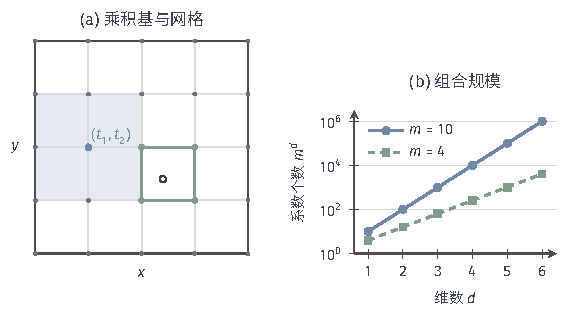
\includegraphics[width=95.0mm]{figures/02-abstract-mathematics/03-function-spaces/tikz/c6-tensor-grid/figure.pdf}
  \caption{张量积网格。(a)~每轴$m=5$个结点，蓝底为乘积帽形基$\varphi_1(x)\varphi_2(y)$的支撑，蓝点为其中心结点$(t_1,t_2)$；空心圆为一个查询点，双线性插值只用它所在单元的四个角点（绿）。(b)~完整张量积系数个数$m^d$随维数$d$指数增长（对数纵轴）。}
  \label{fig:apx-tensor-grid}
\end{figure}

乘积结构也出现在核方法中。第~\ref{sec:rkhs-kernel-operations}节说明两个核的乘积仍是核；$\mathbb R^d$上的高斯核正是$d$个一维高斯核的乘积，其核截面$K_{(x',y')}=K_{1,x'}\otimes K_{2,y'}$是一维核截面的张量积。插值核的频率性质、混叠和实际重建算法属于前面提到的信号问题，这里不展开。

\subsection{低秩分离表示}
\label{sec:apx-low-rank}

完整的张量积展开使用全部$mn$个系数。若系数矩阵近似低秩，就可以只用少数几个乘积项。本小节固定两组变量，研究
\[
  F_r(x,y)=\sum_{j=1}^r u_j(x)v_j(y)
\]
能以什么误差逼近给定的二元函数，其中$r$称为项数。

\paragraph{指数函数的Taylor分离}

以$E(x,y)=e^{xy}$、$(x,y)\in[-1,1]^2$为例。把$t=xy$代入指数函数的Taylor展开并截断，
\begin{equation}
  E_r(x,y)=\sum_{k=0}^{r-1}\frac{x^k y^k}{k!},
  \label{eq:apx-exp-taylor}
\end{equation}
每一项都是$x^k/k!$与$y^k$的乘积，所以$E_r$恰有$r$个分离项。由一元Taylor余项，对$|t|\le1$有$|e^t-\sum_{k<r}t^k/k!|\le e^{|t|}|t|^r/r!\le e/r!$，因此
\[
  \|E-E_r\|_\infty\le\frac{e}{r!}.
\]
实际一致误差在$x=y=1$处取得，等于$e-\sum_{k<r}1/k!$；例如$r=4$时为$e-8/3\approx0.0516$，而上界为$e/24\approx0.113$。图~\ref{fig:apx-lowrank-errors}(a)比较了$r=1,\ldots,8$的实际误差与上界。

这个构造证明了存在一个误差至多$e/r!$的$r$项表示，但没有说明它在所有$r$项表示中是否最好。下面会看到，在$L^2$误差下它并不是最好的。

\paragraph{分离秩无限}

既然每个$E_r$都是有限项，自然要问$E$本身是否也能写成有限个乘积之和。答案是否定的，证明依靠指数和的零点计数。

\begin{lemma}[指数和的零点]
\label{lem:apx-exponential-sum-zeros}
设$\lambda_1<\cdots<\lambda_n$为互异实数，实系数$c_1,\ldots,c_n$不全为零。则$g(t)=\sum_{b=1}^nc_be^{\lambda_bt}$在$\mathbb R$上至多有$n-1$个零点。
\end{lemma}

\begin{proof}
对$n$归纳。$n=1$时$g=c_1e^{\lambda_1t}$没有零点。设结论对$n-1$项成立，不妨设$c_n\ne0$（否则项数更少）。$e^{-\lambda_1t}g(t)=c_1+\sum_{b\ge2}c_be^{(\lambda_b-\lambda_1)t}$与$g$零点相同。若它有$n$个零点，由Rolle定理，其导数$\sum_{b\ge2}c_b(\lambda_b-\lambda_1)e^{(\lambda_b-\lambda_1)t}$至少有$n-1$个零点；这是$n-1$项的指数和，系数$c_n(\lambda_n-\lambda_1)\ne0$，与归纳假设矛盾。
\end{proof}

现在设$e^{xy}=\sum_{j=1}^ru_j(x)v_j(y)$对$x,y\in[-1,1]$成立。取互异点$x_1,\ldots,x_{r+1}$与$y_1,\ldots,y_{r+1}$，矩阵$[e^{x_ay_b}]_{a,b}=\sum_j[u_j(x_a)]_a[v_j(y_b)]_b^{\top}$是$r$个秩一矩阵之和，秩至多为$r$，因而存在非零向量$\bm c$使$\sum_bc_be^{x_ay_b}=0$对$a=1,\ldots,r+1$成立。这说明$r+1$项的指数和$\sum_bc_be^{y_bt}$有$r+1$个零点$x_1,\ldots,x_{r+1}$，与引理~\ref{lem:apx-exponential-sum-zeros}矛盾。因此$e^{xy}$不是任何有限个乘积函数之和，只能被逼近，不能被有限项精确表示。

\paragraph{正交基下的最佳低秩截断}

要找最好的$r$项近似，需要先固定误差范数和允许的因子。设$\{e_i\}_{i=1}^m$与$\{f_k\}_{k=1}^n$分别是$L^2(\mu)$与$L^2(\nu)$中的标准正交组，$F=\sum_{i,k}c_{i,k}e_i\otimes f_k$。由定理~\ref{thm:apx-product-basis}前的计算，$\{e_i\otimes f_k\}$标准正交，所以
\[
  \|F\|_{L^2(\mu\otimes\nu)}=\|\bm C\|_F,
\]
即函数的$L^2$范数等于系数矩阵的Frobenius范数。若因子限制在这两个子空间中，$r$项表示$F_r$的系数矩阵秩至多为$r$，误差$\|F-F_r\|=\|\bm C-\bm C_r\|_F$。由Eckart--Young定理\cite{eckart1936}，最优的$\bm C_r$是$\bm C$的截断奇异值分解，最小误差为$\bigl(\sum_{j>r}\sigma_j^2\bigr)^{1/2}$，$\sigma_j$为$\bm C$的奇异值；矩阵的截断奇异值分解及其最优性可参考\BookChapterRef{chap:matrix-analysis}{卷一“谱和奇异值”章}。

允许因子取遍整个$L^2$空间，并不能做得更好。记$P$、$Q$为到两个子空间的正交投影，则$P\otimes Q$把$r$项表示映成至多$r$项的表示，且$F$在它的值域中，于是
\[
  \|F-F_r\|^2=\|F-(P\otimes Q)F_r\|^2+\|(I-P\otimes Q)F_r\|^2\ge\|F-(P\otimes Q)F_r\|^2 .
\]
最优解总可以取在子空间内。

对$e^{xy}$，取$[-1,1]$上标准正交化的Legendre多项式作基（前$14$个，系数由数值求积计算），奇异值依次约为$2.12$、$0.708$、$0.0892$、$0.00763$、$4.84\times10^{-4}$，迅速衰减。图~\ref{fig:apx-lowrank-errors}(b)比较两种$r$项近似的$L^2$误差：$r=4$时Taylor截断为$9.59\times10^{-3}$，最佳秩$4$截断为$4.85\times10^{-4}$，小约二十倍，而且差距随$r$扩大。

\begin{figure}[!htb]
  \centering
  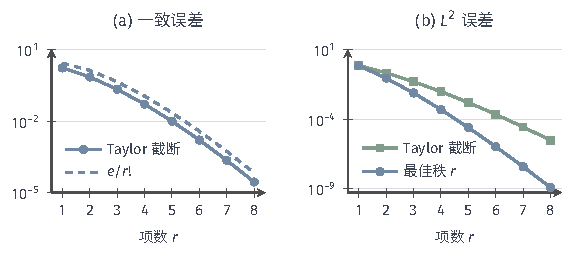
\includegraphics[width=95.9mm]{figures/02-abstract-mathematics/03-function-spaces/tikz/c6-lowrank-errors/figure.pdf}
  \caption{$e^{xy}$在$[-1,1]^2$上的$r$项分离逼近，对数纵轴。(a)~Taylor截断$E_r$的一致误差（实线）与上界$e/r!$（虚线）。(b)~$L^2$误差：Taylor截断（方块）与最佳秩$r$截断（圆点），后者由Legendre正交基下系数矩阵的奇异值算出，为$(\sum_{j>r}\sigma_j^2)^{1/2}$。可行的构造不一定最优。}
  \label{fig:apx-lowrank-errors}
\end{figure}

\paragraph{非正交基与Gram矩阵}

上面的结论依赖基的正交性。若$\bm\varphi$、$\bm\psi$不正交，记Gram矩阵$\bm G_\varphi=[\langle\varphi_i,\varphi_{i'}\rangle]$、$\bm G_\psi=[\langle\psi_k,\psi_{k'}\rangle]$，由式~\eqref{eq:apx-coefficient-matrix}和式~\eqref{eq:apx-product-inner}，
\[
  \|F\|^2=\int\!\!\int\bm\varphi^{\top}\bm C\bm\psi\bm\psi^{\top}\bm C^{\top}\bm\varphi\,\mathrm d\mu\,\mathrm d\nu
  =\operatorname{tr}\bigl(\bm C\bm G_\psi\bm C^{\top}\bm G_\varphi\bigr)
  =\bigl\|\bm G_\varphi^{1/2}\bm C\bm G_\psi^{1/2}\bigr\|_F^2 .
\]
因此最佳截断应作用于加权矩阵$\bm G_\varphi^{1/2}\bm C\bm G_\psi^{1/2}$，截断后再变换回原系数；直接截断$\bm C$的奇异值分解，一般不是$L^2$最优的。

$e^{xy}$恰好是一个例子。在单项式基$\{1,x,x^2,\ldots\}$下，Taylor系数矩阵是对角阵$\operatorname{diag}(1,1,1/2!,1/3!,\ldots)$，它的截断奇异值分解正是Taylor截断$E_r$。单项式基不正交，所以这个截断不是最佳的，图~\ref{fig:apx-lowrank-errors}(b)中两条曲线的差距就来自这里。

\paragraph{项数、因子幅度与高阶情形}

项数$r$、因子的幅度和误差是三个不同的量。同一个乘积可以写成$u\otimes v=(\lambda u)\otimes(v/\lambda)$，因子的大小不由函数决定；两项之差$M\,u\otimes v-M\,u\otimes v'$在$v'$接近$v$时可以很小，而每个因子的范数都含有$M$。只给出项数，既不能控制输出的大小，也不能保证计算稳定。

两组变量的结论依赖矩阵的奇异值分解，不能直接推广到三组及以上的变量。考虑三元函数$T(x,y,z)=x+y+z$，令
\[
  T_n(x,y,z)=n\Bigl(1+\frac xn\Bigr)\Bigl(1+\frac yn\Bigr)\Bigl(1+\frac zn\Bigr)-n .
\]
展开得$T_n=T+(xy+yz+zx)/n+xyz/n^2$，在有界区域上一致收敛到$T$，而每个$T_n$只有两个乘积项（常数$-n$也是乘积函数）。另一方面，$T$不能写成两个三元乘积之和：把任一表示投影到每个变量的$\operatorname{span}\{1,x\}$上，问题化为$2\times2\times2$张量的秩，而对应张量的秩为$3$\scite{desilva2008tensor}。于是$T$到两项表示的距离为零却无法达到，最佳两项近似不存在；逼近列$T_n$的因子幅度还随$n$发散。高阶情形的低秩逼近需要专门的理论，不能套用矩阵截断公式。

% 第8章第3节：函数类的紧性与覆盖数（Arzelà--Ascoli判据、覆盖数与度量熵、覆盖数的估计）。

\section{函数类的紧性与覆盖数}
\label{sec:apx-function-classes}

前两节始终固定一个目标：先给定$f$，再为它挑选近似，近似的预算可以依赖$f$。现在改为预先给定一个函数类$\mathcal F$，要求一套有限的代表同时服务于类中所有成员。量词的次序随之改变：“对每个$f$，存在有限表示”与“存在一套有限代表，对每个$f$都有一个靠近它的代表”是两个不同的命题。后者成立与否，取决于所用的距离以及类中函数共同受到的幅度和正则性约束。

第~\ref{chap:linear-functionals-operators}章的弱紧性不能代替这里的判断。在无限维Hilbert空间中，标准正交序列$(e_n)$有界并弱收敛到零（第~\ref{sec:lfo-weak-subsequence}节），但$\|e_n-e_m\|=\sqrt2$（$n\ne m$），没有按范数收敛的子列，单位球也不能被有限个半径小于$\sqrt2/2$的球覆盖。弱拓扑下的紧性针对较弱的收敛方式；在一致距离或$L^2$距离下能否有限覆盖，需要另外判断。本节先刻画一致距离下的相对紧性，再计量覆盖所需代表的个数。

\subsection{一致有界与等度连续}
\label{sec:apx-arzela-ascoli}

\paragraph{有界不足以抽出一致收敛子列}

在有限维空间中，有界序列总有收敛子列。在$C([0,1])$中这一点不再成立。考虑$f_n(x)=x^n$，它们都满足$\|f_n\|_\infty=1$。逐点地看，$x\in[0,1)$时$x^n\to0$，而$f_n(1)=1$，逐点极限是在$x=1$处跳到$1$的不连续函数。若某个子列一致收敛，其极限连续（一致极限保持连续性，可参考\BookChapterRef{chap:limits-continuity}{卷一“极限与连续”章}），又必须等于逐点极限，这是矛盾。所以$(x^n)$没有一致收敛的子列。

图~\ref{fig:apx-xn-powers}显示了问题出在哪里：$n$越大，函数在$x=1$附近从接近$0$升到$1$所用的区间越窄。每个$x^n$各自连续，但它们的连续性尺度没有共同的下界。

\begin{figure}[!htb]
  \centering
  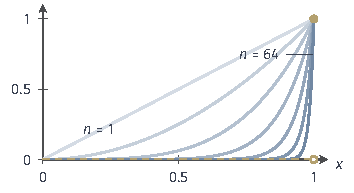
\includegraphics[width=60.0mm]{figures/02-abstract-mathematics/03-function-spaces/tikz/c6-xn-powers/figure.pdf}
  \caption{$[0,1]$上的$x^n$，$n=1,2,4,\ldots,64$（颜色由浅到深）。函数族一致有界，逐点极限在$[0,1)$上为$0$、在$x=1$处为$1$（黄色），不连续，因此没有一致收敛的子列；陡升区间随$n$变窄，族缺少共同的连续性尺度。}
  \label{fig:apx-xn-powers}
\end{figure}

\paragraph{等度连续}

缺少的条件是整个族共用一个连续性尺度。

\begin{definition}[一致有界与等度连续]
\label{def:apx-equicontinuous}
设$(X,d)$是度量空间，$\mathcal F$是$X$上的一族实值函数。若存在$M$使$|f(x)|\le M$对所有$f\in\mathcal F$、$x\in X$成立，称$\mathcal F$\term{一致有界}（uniformly bounded）。若对每个$\varepsilon>0$存在$\delta>0$，使
\[
  d(x,y)<\delta\ \Longrightarrow\ |f(x)-f(y)|<\varepsilon\qquad\text{对所有}f\in\mathcal F,
\]
称$\mathcal F$\term{等度连续}（equicontinuous）。
\end{definition}

与单个函数的一致连续相比，关键在于$\delta$只依赖$\varepsilon$，不依赖$f$。用连续模的语言，等度连续就是$\sup_{f\in\mathcal F}\omega_f(\delta)\to0$。最常见的例子是共用一个Lipschitz常数的族：若每个$f\in\mathcal F$都满足$|f(x)-f(y)|\le Ld(x,y)$，取$\delta=\varepsilon/L$即可。

反例来自没有共同尺度的族。$(x^n)$不等度连续：对任意$\delta\in(0,1)$，取$x=1$、$y=1-\delta/2$，则$|f_n(x)-f_n(y)|=1-(1-\delta/2)^n\to1$。图~\ref{fig:apx-equicontinuity}比较了两族函数在同一个宽$0.1$的窗口内的振幅：(a)中四个函数的Lipschitz常数都是$0.8\pi$，窗口内振幅都不超过$0.26$；(b)中$0.5+0.5\sin(2\pi nx)$的频率增长，$n=16$时在窗口内已扫过整个$[0,1]$。

\begin{figure}[!htb]
  \centering
  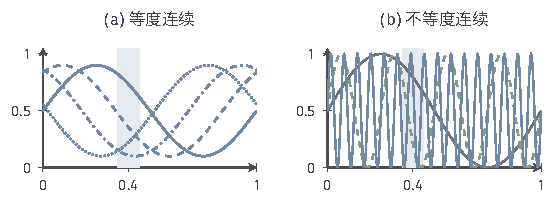
\includegraphics[width=94.2mm]{figures/02-abstract-mathematics/03-function-spaces/tikz/c6-equicontinuity/figure.pdf}
  \caption{共同连续性尺度的有无。蓝底为窗口$[0.35,0.45]$。(a)~$0.5+0.4\sin(2\pi x+a)$，$a=0,1,2,3$，共用Lipschitz常数$0.8\pi$，窗口内振幅都不超过$0.26$，族等度连续。(b)~$0.5+0.5\sin(2\pi nx)$，$n=1,4,16$，频率越高窗口内振幅越大，$n=16$时已达到$1$，族不等度连续。}
  \label{fig:apx-equicontinuity}
\end{figure}

\paragraph{Arzelà--Ascoli判据}

在紧度量空间上，一致有界与等度连续恰好刻画了一致距离下的相对紧性。回忆$C(X)$在一致范数下完备（第~\ref{sec:fs-uniform-norm}节）；子集称为\term{相对紧}（relatively compact），若它的闭包是紧集。

\begin{theorem}[Arzelà--Ascoli判据]
\label{thm:apx-arzela-ascoli}
设$(X,d)$是非空紧度量空间，$\mathcal F\subseteq C(X)$。则$\mathcal F$在一致范数下相对紧，当且仅当$\mathcal F$一致有界且等度连续。若$\mathcal F$还是闭集，则它是紧集。
\end{theorem}

证明的核心是一个有限化的机制：等度连续允许只在有限个位置上观察函数，一致有界允许把这些位置上的值量化为有限个等级，于是整个族只产生有限种“记录”。

\begin{proof}
充分性。设$|f|\le M$对所有$f\in\mathcal F$成立，并给定$\varepsilon>0$。由等度连续取$\delta>0$，使$d(x,y)<\delta$时$|f(x)-f(y)|<\varepsilon/4$对所有$f$成立。$X$紧，因而全有界，存在有限个点$x_1,\ldots,x_p$，使每个$x$都满足某个$d(x,x_i)<\delta$。再把$[-M,M]$分成有限个长度为$\varepsilon/4$的左闭右开小区间（最后一段含右端点），对每个$f$记下$f(x_1),\ldots,f(x_p)$各落在哪个小区间，称为$f$的记录。记录至多有$(\lceil8M/\varepsilon\rceil)^p$种，是有限个。

对每一种实际出现的记录，从$\mathcal F$中取一个具有该记录的成员作为代表。若$f$与代表$g$记录相同，则$|f(x_i)-g(x_i)|<\varepsilon/4$对每个$i$成立。对任意$x$取$x_i$使$d(x,x_i)<\delta$，
\[
  |f(x)-g(x)|\le|f(x)-f(x_i)|+|f(x_i)-g(x_i)|+|g(x_i)-g(x)|<\frac{3\varepsilon}4 .
\]
因此有限个代表构成$\mathcal F$的有限$\varepsilon$网，$\mathcal F$全有界。全有界集的闭包仍全有界（把每个球的半径放大一倍即可），而闭包是完备空间$C(X)$的闭子集，因而完备。由定理~\ref{thm:metric-compact-complete-tb}，闭包紧致。

必要性。设$\overline{\mathcal F}$紧，则$\mathcal F$全有界。取有限$\varepsilon/3$网$f_1,\ldots,f_N\in\mathcal F$。有界性：每个$f$都在某个$f_j$的$\varepsilon/3$邻域内，故$\|f\|_\infty\le\max_j\|f_j\|_\infty+\varepsilon/3$。等度连续：每个$f_j$在紧集上一致连续（定理~\ref{thm:metric-compact-uniform}），取$\delta$对这有限个函数同时适用，使$d(x,y)<\delta$时$|f_j(x)-f_j(y)|<\varepsilon/3$。对任意$f$选$f_j$使$\|f-f_j\|_\infty<\varepsilon/3$，则
\[
  |f(x)-f(y)|\le|f(x)-f_j(x)|+|f_j(x)-f_j(y)|+|f_j(y)-f(y)|<\varepsilon .
\]
最后，若$\mathcal F$闭，则$\mathcal F=\overline{\mathcal F}$紧。
\end{proof}

必要性的论证说明了有限网的作用：有限个函数总能共用一个$\delta$，再借助一致距离把这个$\delta$传给整个族。充分性中的位置网格和数值量化则是一个可以计数的构造，第~\ref{sec:apx-covering-estimates}节将用它给出Lipschitz类覆盖数的显式上界，图~\ref{fig:apx-lipschitz-quantization}画出了这个构造。

\paragraph{核范数有界球的一致紧性}

第~\ref{chap:rkhs}章的两个不等式恰好提供了Arzelà--Ascoli判据的两个条件。设$X$是紧度量空间，$K$是$X$上的连续半正定核，$B_R=\{f\in H_K:\|f\|_{H_K}\le R\}$。

\begin{theorem}[核范数球在连续函数空间中的紧性]
\label{thm:apx-rkhs-ball-compact}
在上述条件下，$B_R$是$C(X)$中按一致范数的紧集。
\end{theorem}

\begin{proof}
一致有界：由点值界（第~\ref{sec:rkhs-kernel-properties}节），$|f(x)|\le\|f\|_{H_K}\sqrt{K(x,x)}\le R\max_{X}\sqrt{K(x,x)}$，右端有限，因为连续函数在紧集上有最大值。

等度连续：由再生关系，
\[
  \begin{aligned}
  |f(x)-f(y)|&=|\langle f,K_x-K_y\rangle_{H_K}|\le R\,\|K_x-K_y\|_{H_K}\\
  &=R\sqrt{K(x,x)+K(y,y)-2K(x,y)} .
  \end{aligned}
\]
右端是$X\times X$上的连续函数，在对角线上为零。它在紧集$X\times X$上一致连续，所以存在$\delta$，使$d(x,y)<\delta$时右端小于$\varepsilon$，且$\delta$与$f\in B_R$无关。这里同时得到$B_R\subseteq C(X)$。

闭性：设$f_n\in B_R$且一致收敛到$g\in C(X)$。$(f_n)$在$H_K$中有界，由第~\ref{sec:lfo-weak-subsequence}节，存在子列弱收敛到某个$h\in H_K$；弱极限的范数不超过序列范数的下极限（第~\ref{sec:lfo-weak-norm}节），故$\|h\|_{H_K}\le R$。弱收敛蕴含$f_{n_k}(x)=\langle f_{n_k},K_x\rangle\to\langle h,K_x\rangle=h(x)$，而$f_{n_k}(x)\to g(x)$，所以$g=h\in B_R$。由定理~\ref{thm:apx-arzela-ascoli}，$B_R$紧。
\end{proof}

这个定理改变的是评价距离。$B_R$在一致距离下紧，并不意味着它在$H_K$自身的范数下紧：若$H_K$无限维，取其中的标准正交序列$(e_n)$，它们都在$B_1$中，彼此的核范数距离为$\sqrt2$，没有核范数收敛的子列。$[0,1]$上的高斯核就是这种情形：对互异中心$c_1,\ldots,c_M$，若$\sum_\ell a_\ell K_\sigma(\cdot,c_\ell)\equiv0$，乘以$e^{x^2/(2\sigma^2)}$后得到指数和$\sum_\ell a_\ell e^{-c_\ell^2/(2\sigma^2)}e^{c_\ell x/\sigma^2}\equiv0$，由引理~\ref{lem:apx-exponential-sum-zeros}全部$a_\ell=0$，所以$H_K$含有任意多个线性无关元素。

定理~\ref{thm:apx-rkhs-ball-compact}也补全了第~\ref{sec:apx-kernel-sections}节留下的论断：$B_R$在$C([0,1])$中闭且只含$H_K$的元素，$f_*\notin H_K$，所以$f_*$到$B_R$有正的一致距离。对任何固定的核范数预算$R$，有限核和都不能任意逼近$f_*$。

\subsection{覆盖数与度量熵}
\label{sec:apx-covering}

紧性回答“能否用有限个代表统一逼近”，没有回答“需要多少个”。本小节把代表的个数作为精度的函数记录下来。

\paragraph{覆盖数的定义与量词}

\begin{definition}[覆盖数与度量熵]
\label{def:apx-covering-number}
设$\mathcal F$是非空集合，$d$是$\mathcal F$上的距离或伪距离，$\varepsilon>0$。若有限集$V\subseteq\mathcal F$使每个$f\in\mathcal F$都有$v\in V$满足$d(f,v)\le\varepsilon$，称$V$为$\mathcal F$的一个$\varepsilon$覆盖。最小的覆盖规模
\[
  N(\varepsilon,\mathcal F,d)=\min\bigl\{|V|:V\text{是}\mathcal F\text{的}\varepsilon\text{覆盖}\bigr\}
\]
称为\term{覆盖数}（covering number），不存在有限覆盖时记为$+\infty$。其对数$\log N(\varepsilon,\mathcal F,d)$称为\term{度量熵}（metric entropy）。
\end{definition}

定义的量词是
\[
  \exists\ \text{有限}\ V\subseteq\mathcal F,\quad\forall f\in\mathcal F,\quad\exists v\in V:\ d(f,v)\le\varepsilon .
\]
代表集$V$必须在看到具体的$f$之前就固定下来，而且对类中每个成员都有效；只对大多数成员有效、或平均意义下有效，都不满足要求。每个$f$可以选择自己的近邻代表，但只能从$V$中选。

这里约定代表属于$\mathcal F$本身。若允许代表取自更大的空间，所得的外部覆盖数$N^{\mathrm{ext}}$可能更小，但两者只差精度的一个因子：
\[
  N^{\mathrm{ext}}(\varepsilon)\le N(\varepsilon)\le N^{\mathrm{ext}}(\varepsilon/2).
\]
第一个不等式显然。第二个：取一个外部$\varepsilon/2$覆盖，对每个与$\mathcal F$相交的球选一个类内成员替换球心，由三角不等式，原来落在该球中的成员到新代表的距离不超过$\varepsilon$。比较不同文献中的数值时，要先核对采用的是哪种约定。

\paragraph{覆盖数与全有界、紧性}

覆盖数把全有界的定义量化了。$\mathcal F$在$d$下全有界（定义~\ref{def:metric-totally-bounded}），当且仅当对每个$\varepsilon>0$都有$N(\varepsilon,\mathcal F,d)<\infty$：闭球$\{d(f,v)\le\varepsilon/2\}$含于开球$\{d(f,v)<\varepsilon\}$，开球又含于同半径的闭球，所以开球与闭球给出的有限性相同。若$\mathcal F$位于一个完备度量空间中，由定理~\ref{thm:metric-compact-complete-tb}，覆盖数处处有限等价于$\mathcal F$相对紧。结合定理~\ref{thm:apx-arzela-ascoli}，紧度量空间上一致有界且等度连续的函数族，在一致距离下对每个精度都有有限覆盖数。

伪距离允许$d(f,g)=0$而$f\ne g$。此时覆盖数只计及零距离等价类：彼此距离为零的成员共用同一个代表，因此应在第~\ref{sec:metric-pseudometric}节的商空间上理解覆盖数及其与紧性的关系。

\paragraph{三种距离的比较}

同一个函数类在不同距离下的覆盖数可以截然不同。设$X$上有概率测度$\mu$，又固定样本点$x_1,\ldots,x_n\in X$。三个常用的距离或伪距离为
\[
  \begin{aligned}
  d_\infty(f,g)&=\sup_{x\in X}|f(x)-g(x)|,\qquad
  d_{L^2(\mu)}(f,g)=\|f-g\|_{L^2(\mu)},\\
  d_n(f,g)&=\Bigl(\frac1n\sum_{i=1}^n\bigl(f(x_i)-g(x_i)\bigr)^2\Bigr)^{1/2}.
  \end{aligned}
\]
由于$\mu(X)=1$，后两者都不超过$d_\infty$。距离越弱，$\varepsilon$球越大，因此
\[
  N(\varepsilon,\mathcal F,d_{L^2(\mu)})\le N(\varepsilon,\mathcal F,d_\infty),\qquad
  N(\varepsilon,\mathcal F,d_n)\le N(\varepsilon,\mathcal F,d_\infty).
\]

经验距离$d_n$只看样本点，所以通常只是伪距离。图~\ref{fig:apx-empirical-distance}中$g(x)=0.3+0.4x$与$f(x)=g(x)+0.35\sin(5\pi x)$在六个样本点$0,0.2,\ldots,1$处取值相同，$d_n(f,g)=0$，但$d_\infty(f,g)=0.35$。

\begin{figure}[!htb]
  \centering
  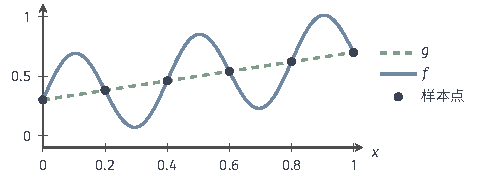
\includegraphics[width=81.2mm]{figures/02-abstract-mathematics/03-function-spaces/tikz/c6-empirical-distance/figure.pdf}
  \caption{经验距离只看样本点。$g(x)=0.3+0.4x$（虚线）与$f(x)=g(x)+0.35\sin(5\pi x)$（实线）在样本点$0,0.2,\ldots,1$（黑点）处相等，经验距离为$0$，一致距离却为$0.35$。}
  \label{fig:apx-empirical-distance}
\end{figure}

反方向的比较不成立，而且差距可以是有限与无穷之别。令$\mathcal F$为全体取值于$[0,1]$的连续函数。在$d_n$下，每个$f$由向量$(f(x_1),\ldots,f(x_n))\in[0,1]^n$决定距离；把每个坐标量化到$\lceil1/(2\varepsilon)\rceil$个等距点之一，所得网格点都是某个连续函数的样本值，于是$N(\varepsilon,\mathcal F,d_n)\le\lceil1/(2\varepsilon)\rceil^n<\infty$。在$d_\infty$下，取支撑互不相交的帽形函数列$(\phi_k)$，峰值为$1$，则$d_\infty(\phi_k,\phi_l)=1$（$k\ne l$），任何半径$1/3$的球至多含其中一个，所以$N(1/3,\mathcal F,d_\infty)=\infty$。样本上的记录有限，不能推出整个定义域上的有限覆盖；要从有限位置控制全域，需要等度连续这样的共同正则性，这正是定理~\ref{thm:apx-arzela-ascoli}的作用。

\subsection{覆盖数的估计与适用范围}
\label{sec:apx-covering-estimates}

本小节对几类具体的函数类估计覆盖数，观察它怎样依赖函数的幅度、参数维数、正则性和定义域。

\paragraph{常值族}

先看最简单的一维情形。设$X$非空，$M>0$，$\mathcal F_M=\{f_a\equiv a:a\in[0,M]\}$，距离取$d_\infty$。两个常值函数的距离就是$|a-a'|$，所以问题化为用半径$\varepsilon$的闭区间覆盖$[0,M]$。

下界由长度比较给出：每个代表$c$只覆盖长度为$2\varepsilon$的参数区间$[c-\varepsilon,c+\varepsilon]$，$N$个代表覆盖的总长度至多$2N\varepsilon$，必须不小于$M$。上界由均匀分点给出：令$N=\lceil M/(2\varepsilon)\rceil$，取$c_j=(2j-1)M/(2N)$，$j=1,\ldots,N$，相邻代表间距为$M/N\le2\varepsilon$，每个参数到最近代表的距离不超过$M/(2N)\le\varepsilon$。因此
\[
  N(\varepsilon,\mathcal F_M,d_\infty)=\Bigl\lceil\frac{M}{2\varepsilon}\Bigr\rceil,
\]
图~\ref{fig:apx-constant-cover}画出$M=1$、$\varepsilon=0.15$时的四个代表。

\begin{figure}[!htb]
  \centering
  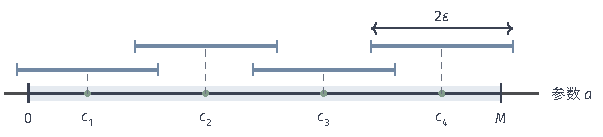
\includegraphics[width=102.2mm]{figures/02-abstract-mathematics/03-function-spaces/tikz/c6-constant-cover/figure.pdf}
  \caption{常值族$f_a\equiv a$（$a\in[0,1]$）在一致距离下的覆盖，精度$\varepsilon=0.15$。每个代表$c_j$（绿点）只覆盖长度$2\varepsilon$的参数区间（蓝色线段，上下错开以便辨认）；四个代表的总长度$1.2$不小于$1$，而三个只有$0.9$，所以覆盖数恰为$\lceil1/(2\varepsilon)\rceil=4$。}
  \label{fig:apx-constant-cover}
\end{figure}

这个例子已经显示了幅度的作用。参数个数固定为一个，把幅度$M$放大，覆盖数随$M$线性增长；一般地，对任意类$\mathcal F$和$B>0$，$N(\varepsilon,B\mathcal F,d_\infty)=N(\varepsilon/B,\mathcal F,d_\infty)$。度量熵$\log\lceil M/(2\varepsilon)\rceil$则只按$\log(1/\varepsilon)$增长。

\paragraph{有限维参数族}

再看两个参数的情形。设$\mathcal F=\{f_{a,b}(t)=a+bt:(a,b)\in[-1,1]^2\}$，$t\in[-1,1]$，距离取$d_\infty$。差$(a-a')+(b-b')t$是$t$的一次函数，绝对值的最大值在端点取得，等于$|a-a'|+|b-b'|$。因此一致距离恰好是系数平面上的$\ell^1$距离，$\varepsilon$球是菱形。

上界：把$[-1,1]$等分为$\lceil2/\varepsilon\rceil$段，取各段中点，每段长度不超过$\varepsilon$，所以每个坐标到最近中点的距离不超过$\varepsilon/2$。两个坐标方向的中点组成网格，每个系数点到最近网格点的$\ell^1$距离不超过$\varepsilon$，故$N(\varepsilon)\le\lceil2/\varepsilon\rceil^2$。下界：每个菱形面积为$2\varepsilon^2$，覆盖面积为$4$的正方形至少需要$4/(2\varepsilon^2)=2/\varepsilon^2$个。于是
\[
  \frac2{\varepsilon^2}\le N(\varepsilon,\mathcal F,d_\infty)\le\Bigl\lceil\frac2\varepsilon\Bigr\rceil^2,
\]
覆盖数按$\varepsilon^{-2}$增长，指数$2$正是参数个数。图~\ref{fig:apx-covering-centers}画出$\varepsilon=1/2$时的$16$个代表：(a)是系数平面上的菱形覆盖，(b)是对应的函数。

\begin{figure}[!htb]
  \centering
  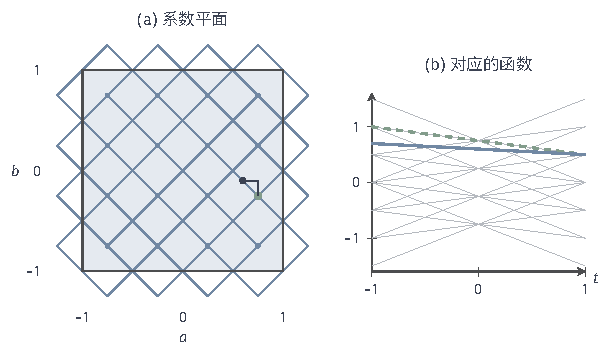
\includegraphics[width=103.2mm]{figures/02-abstract-mathematics/03-function-spaces/tikz/c6-covering-centers/figure.pdf}
  \caption{仿射函数类$a+bt$（$(a,b)\in[-1,1]^2$，$t\in[-1,1]$）的$\tfrac12$覆盖。(a)~一致距离等于系数的$\ell^1$距离，$16$个中心$\{\pm\frac14,\pm\frac34\}^2$的半径$\frac12$菱形覆盖整个正方形；黑点$(0.6,-0.1)$到最近中心$(\frac34,-\frac14)$（绿）的$\ell^1$距离为$0.3$。(b)~对应的函数：$16$条中心直线（细灰），成员$0.6-0.1t$（蓝）与其代表$0.75-0.25t$（绿虚线）的一致距离为$0.3$，在$t=-1$处取得。}
  \label{fig:apx-covering-centers}
\end{figure}

同样的论证适用于一般的有限维参数族。设$\mathcal F=\{\sum_{i=1}^p\theta_i\varphi_i:\|\bm\theta\|_\infty\le B\}$，$\varphi_i$有界，令$\Lambda=\sup_x\sum_i|\varphi_i(x)|$。则$d_\infty(f_{\bm\theta},f_{\bm\theta'})\le\Lambda\|\bm\theta-\bm\theta'\|_\infty$，把参数立方体$[-B,B]^p$在每个坐标上按精度$\varepsilon/\Lambda$分点，得到
\[
  N(\varepsilon,\mathcal F,d_\infty)\le\Bigl\lceil\frac{B\Lambda}\varepsilon\Bigr\rceil^p,\qquad
  \log N\le p\log\Bigl\lceil\frac{B\Lambda}\varepsilon\Bigr\rceil .
\]
若$\varphi_i$线性无关，有限维空间上的范数等价给出反方向的比较，再用体积论证可以得到同阶的下界，这里不展开。

\paragraph{参数个数不是覆盖数}

上面的例子中覆盖数的指数等于参数个数，但这是因为参数与函数一一对应且距离可以互相比较。覆盖数衡量的是函数集合本身在所选距离下的大小，与怎样参数化无关。把常值族改写成$f_{\theta_1,\theta_2}=\theta_1+\theta_2$，$\theta_1,\theta_2\in[0,M/2]$，参数变成两个，函数集合仍是$\{a:a\in[0,M]\}$，覆盖数不变。反过来，取$f_\theta\equiv\sin(M\theta)$，$\theta\in[0,2\pi]$，$M$为正整数：参数只有一个，参数到函数的映射随$M$增大而变得剧烈，但函数集合始终是取值于$[-1,1]$的常值函数，覆盖数$\lceil1/\varepsilon\rceil$与$M$无关。参数个数、参数化的剧烈程度和函数类的大小，是三个需要分别判断的量。

\paragraph{Lipschitz类的网格量化覆盖}

最后回到Arzelà--Ascoli判据证明中的构造，把它变成显式的计数。

\begin{theorem}[Lipschitz类的覆盖数上界]
\label{thm:apx-lipschitz-covering}
设$(X,d)$是非空紧度量空间，$L,M>0$，
\[
  \mathcal F_{L,M}=\bigl\{f:X\to\mathbb R:\ |f|\le M,\ |f(x)-f(y)|\le Ld(x,y)\bigr\}.
\]
则对每个$\varepsilon>0$，
\[
  N(\varepsilon,\mathcal F_{L,M},d_\infty)\le\Bigl\lceil\frac{4M}{\varepsilon}\Bigr\rceil^{p},\qquad
  p=N\Bigl(\frac{\varepsilon}{4L},X,d\Bigr).
\]
\end{theorem}

\begin{proof}
令$\delta=\varepsilon/(4L)$，$\eta=\varepsilon/2$。取$X$的一个$\delta$覆盖$x_1,\ldots,x_p$，使每个$x$都有$d(x,x_i)\le\delta$。把$[-M,M]$分成$\lceil2M/\eta\rceil=\lceil4M/\varepsilon\rceil$个长度不超过$\eta$的左闭右开小区间（最后一段含右端点），称$f$在各网格点处的值所在的小区间组成的序列为$f$的记录。记录至多有$\lceil4M/\varepsilon\rceil^p$种。

对每种实际出现的记录，取$\mathcal F_{L,M}$中一个具有该记录的成员作为代表。若$f$与代表$g$记录相同，则$|f(x_i)-g(x_i)|<\eta$。对任意$x$取$x_i$使$d(x,x_i)\le\delta$，
\[
  |f(x)-g(x)|\le Ld(x,x_i)+|f(x_i)-g(x_i)|+Ld(x_i,x)<2L\delta+\eta=\varepsilon .
\]
所以这些代表构成$\varepsilon$覆盖。
\end{proof}

图~\ref{fig:apx-lipschitz-quantization}以$L=1$、$M=0.6$、$\varepsilon=0.4$为例：$\delta=0.1$，网格点取$0.1,0.3,0.5,0.7,0.9$（$p=5$），值域按$\eta=0.2$分层，共$6$层，上界为$6^5=7776$。图中两个函数在每个网格点处落在同一层，一致距离约为$0.16$，不超过$0.4$。

\begin{figure}[!htb]
  \centering
  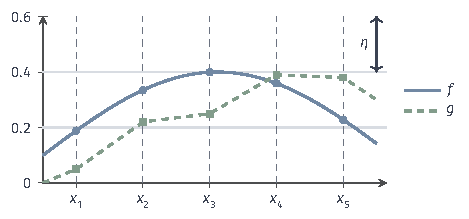
\includegraphics[width=79.4mm]{figures/02-abstract-mathematics/03-function-spaces/tikz/c6-lipschitz-quantization/figure.pdf}
  \caption{Lipschitz类的网格量化，$L=1$，$\varepsilon=0.4$。竖虚线为网格点$x_1,\ldots,x_5$，相邻间距$2\delta=0.2$，每点到最近网格点不超过$\delta=\varepsilon/(4L)$；横线把值域分为高$\eta=\varepsilon/2$的层（图中只画出非负部分）。$f(x)=0.1+0.3\sin3x$（蓝）与折线$g$（绿）在每个网格点处落在同一层，即记录相同，二者一致距离不超过$2L\delta+\eta=\varepsilon$。}
  \label{fig:apx-lipschitz-quantization}
\end{figure}

定义域的覆盖数出现在指数上。对$X=[0,1]$，$p=\lceil1/(2\delta)\rceil=\lceil2L/\varepsilon\rceil$，得到
\[
  \log N(\varepsilon,\mathcal F_{L,M},d_\infty)\le\Bigl\lceil\frac{2L}\varepsilon\Bigr\rceil\log\Bigl\lceil\frac{4M}\varepsilon\Bigr\rceil .
\]
与有限维参数族的$p\log(1/\varepsilon)$相比，这里的“有效维数”$\lceil2L/\varepsilon\rceil$随精度增长，Lipschitz类是无限维的。对$X=[0,1]^d$，网格点个数按$(L/\varepsilon)^d$增长，度量熵也随之增长，这是与张量积网格同源的维数效应。这个上界并不最优：Kolmogorov与Tikhomirov证明，固定$L$、$M$时，$[0,1]^d$上有界Lipschitz类的度量熵在$\varepsilon\to0$时与$\varepsilon^{-d}$同阶，上界中多出的对数因子可以去掉\scite{kolmogorov1959epsilon}。这里的构造只用来说明有限覆盖如何从共同的正则性和幅度约束中产生。

\paragraph{覆盖数之外的容量与保证}

覆盖数总是相对于一个预先固定的距离和精度定义的。学习理论中还会遇到其他容量量：伪维和胖打散维数检查一个类在有限输入上能实现多少种跨越阈值的模式，序贯覆盖数在依赖历史的查询树上计数。它们的评价对象与覆盖数不同，不能从名称相近而互换。覆盖数本身也不提供统计误差或预测保证；要得到这类结论，还需加入随机样本、损失函数和集中不等式，可参考\BookChapterRef{chap:statistical-learning-framework}{卷六“机器学习理论基础”章}。

% 第8章第4节：本章小结（同时收束“函数空间”部分）。

\section{本章小结}
\label{sec:apx-summary}

章首提出的三个问题，分别对应逼近对象的三个层次。

对一个给定的函数，逼近的含义取决于固定了什么：定义域、误差范数和生成单元。Bernstein多项式、线性样条、固定宽度的高斯核截面和单隐藏层网络都能一致逼近紧集上的任意连续目标，但这些都是可变预算下的存在性结论，次数、结点、中心或单元数随精度增加。误差随预算下降的速度另需光滑性：连续模给出$\omega_f(h)$量级，二阶导数有界给出$h^2$量级，折线$f_*$只有一阶。稠密性还不等于能稳定地算出系数：高斯核和的系数可能随精度发散，在固定核范数预算下甚至无法任意逼近$f_*$；网络参数也不可识别。

对多变量函数，乘积结构提供了组合的方式。在可分的$L^2$空间中，单变量正交基的乘积构成乘积测度下的正交基，张量积网格却使系数个数按$m^d$增长。低秩表示只保留少数乘积项；在正交基下，最佳$r$项$L^2$近似由系数矩阵的截断奇异值分解给出，非正交基须先计入Gram矩阵。项数、因子幅度与误差是不同的量，三组以上变量时最佳低秩近似甚至可能不存在。

对整个函数类，量词从“对每个目标存在近似”变为“存在一套代表适用于全体”。一致距离下，紧度量空间上的函数族相对紧，当且仅当一致有界且等度连续；核范数有界球因点值界与核截面差界而在$C(X)$中紧，却不在核范数下紧。覆盖数计量所需代表的个数，它依赖所选的距离：经验距离下的有限覆盖不能推出全域覆盖。常值族、有限维参数族与Lipschitz类的估计表明，覆盖数随幅度、参数维数、正则性和定义域维数变化，而不由参数个数单独决定。

至此，本部分建立了研究函数的几套工具：第~\ref{chap:function-spaces}章的范数、完备性与正交几何，第~\ref{chap:linear-functionals-operators}章与第~\ref{chap:operator-spectra-equations}章的泛函、算子、谱与方程，第~\ref{chap:weak-derivatives-sobolev}章以弱导数刻画的正则性，第~\ref{chap:rkhs}章以点值观测构造的核空间，以及本章的有限逼近与覆盖。它们回答的是候选函数在什么空间中、怎样度量、怎样表示和能逼近到什么程度。后续的优化问题在这些候选空间上加入目标函数与约束，研究最优解的存在、最优条件和求解方法，可参考\BookChapterRef{chap:optimization}{卷三“优化问题的定义与基本性质”章}；信号处理加入时间、频率和采样机制；统计与学习理论加入随机数据和误差保证。它们沿用这里已经确定的范数、表示与覆盖结论，只在各自的问题中补充新的结构。

